%!TEX root = ../main.tex
% \textit{[Lezione 10 (02-04-2020)]}

\chapter{Approssimazione di funzioni e dati}

L'obiettivo di un'approssimazione funzionale è sostituire una funzione \textit{complicata} con una funzione \textit{semplice} ricercata in una classe prefissata di funzioni, in genere dei polinomi.

\textit{Esempio.} L'espressione analitica di una funzione $f$ non è nota, ma essa è solo campionata, ovvero il suo valore è noto solamente su un insieme di punti $x_0, \dots, x_n$, e vogliamo determinare una possibile espressione di $f$.

\begin{figure}[htpb]
	\centering
	\tikzset{every picture/.style={line width=0.75pt}} %set default line width to 0.75pt

	\begin{tikzpicture}[x=0.75pt,y=0.75pt,yscale=-1,xscale=1]
	%uncomment if require: \path (0,216); %set diagram left start at 0, and has height of 216

	%Shape: Axis 2D [id:dp7681657976935359]
	\draw  (234,173.52) -- (508.5,173.52)(261.45,36.17) -- (261.45,188.78) (501.5,168.52) -- (508.5,173.52) -- (501.5,178.52) (256.45,43.17) -- (261.45,36.17) -- (266.45,43.17)  ;
	%Curve Lines [id:da48740805964175427]
	\draw  [dash pattern={on 0.84pt off 2.51pt}]  (245.5,144.78) .. controls (312,51.17) and (432,179.17) .. (489,58.17) ;
	%Straight Lines [id:da43786339887025716]
	\draw    (293,168.59) -- (293,178) ;
	%Straight Lines [id:da023194448258216926]
	\draw    (333,168.59) -- (333,178) ;
	%Straight Lines [id:da8232346787407612]
	\draw    (373,168.59) -- (373,178) ;
	%Straight Lines [id:da4457891900858195]
	\draw    (473,168.59) -- (473,178) ;
	%Shape: Circle [id:dp24863242874775415]
	\draw  [draw opacity=0][fill={rgb, 255:red, 0; green, 0; blue, 0 }  ,fill opacity=1 ] (291,110.59) .. controls (291,109.49) and (291.9,108.59) .. (293,108.59) .. controls (294.1,108.59) and (295,109.49) .. (295,110.59) .. controls (295,111.7) and (294.1,112.59) .. (293,112.59) .. controls (291.9,112.59) and (291,111.7) .. (291,110.59) -- cycle ;
	%Shape: Circle [id:dp914917520550603]
	\draw  [draw opacity=0][fill={rgb, 255:red, 0; green, 0; blue, 0 }  ,fill opacity=1 ] (331,107.59) .. controls (331,106.49) and (331.9,105.59) .. (333,105.59) .. controls (334.1,105.59) and (335,106.49) .. (335,107.59) .. controls (335,108.7) and (334.1,109.59) .. (333,109.59) .. controls (331.9,109.59) and (331,108.7) .. (331,107.59) -- cycle ;
	%Shape: Circle [id:dp6230329978907112]
	\draw  [draw opacity=0][fill={rgb, 255:red, 0; green, 0; blue, 0 }  ,fill opacity=1 ] (371,112.59) .. controls (371,111.49) and (371.9,110.59) .. (373,110.59) .. controls (374.1,110.59) and (375,111.49) .. (375,112.59) .. controls (375,113.7) and (374.1,114.59) .. (373,114.59) .. controls (371.9,114.59) and (371,113.7) .. (371,112.59) -- cycle ;
	%Shape: Circle [id:dp7316490236444106]
	\draw  [draw opacity=0][fill={rgb, 255:red, 0; green, 0; blue, 0 }  ,fill opacity=1 ] (471,83.59) .. controls (471,82.49) and (471.9,81.59) .. (473,81.59) .. controls (474.1,81.59) and (475,82.49) .. (475,83.59) .. controls (475,84.7) and (474.1,85.59) .. (473,85.59) .. controls (471.9,85.59) and (471,84.7) .. (471,83.59) -- cycle ;

	% Text Node
	\draw (244,16.4) node [anchor=north west][inner sep=0.75pt]    {$y$};
	% Text Node
	\draw (523,166.4) node [anchor=north west][inner sep=0.75pt]    {$x$};
	% Text Node
	\draw (285,180.4) node [anchor=north west][inner sep=0.75pt]    {$x_{0}$};
	% Text Node
	\draw (325,180.4) node [anchor=north west][inner sep=0.75pt]    {$x_{1}$};
	% Text Node
	\draw (365,180.4) node [anchor=north west][inner sep=0.75pt]    {$x_{2}$};
	% Text Node
	\draw (465,180.4) node [anchor=north west][inner sep=0.75pt]    {$x_{n}$};
	% Text Node
	\draw (75,60.4) node [anchor=north west][inner sep=0.75pt]    {$\begin{array}{ c|c }
	x & f( x)\\
	\hline
	x_{0} & y_{0} =f( x_{0})\\
	x_{1} & y_{1} =f( x_{1})\\
	\vdots  & \vdots \\
	x_{n} & y_{n} =f( x_{n})
	\end{array}$};
	% Text Node
	\draw (413,179.4) node [anchor=north west][inner sep=0.75pt]    {$\dotsc $};


	\end{tikzpicture}
	\caption{Esempio monodimensionale in cui conosciamo il valore della funzione, solo in alcuni punti, ma vogliamo in qualche modo determinarne un'approssimazione. La linea tratteggiata indica una delle tante possibilità di $f$, infatti passa per tutti i campionamenti.}
	\label{fig:esempio-campionamento}
\end{figure}
\FloatBarrier

\textit{Esempio.} Conosciamo l'espressione analitica di $f$, ma vogliamo sostituirla con una funzione più \textit{semplice} per il calcolo numerico oppure, ad esempio, per rendere possibili o più semplici delle operazioni funzionali quali l'integrazione o la derivazione.

% Pattern Info

\begin{figure}[htpb]
	\centering
	\tikzset{
	pattern size/.store in=\mcSize,
	pattern size = 5pt,
	pattern thickness/.store in=\mcThickness,
	pattern thickness = 0.3pt,
	pattern radius/.store in=\mcRadius,
	pattern radius = 1pt}
	\makeatletter
	\pgfutil@ifundefined{pgf@pattern@name@_5a3929o9p}{
	\pgfdeclarepatternformonly[\mcThickness,\mcSize]{_5a3929o9p}
	{\pgfqpoint{0pt}{-\mcThickness}}
	{\pgfpoint{\mcSize}{\mcSize}}
	{\pgfpoint{\mcSize}{\mcSize}}
	{
	\pgfsetcolor{\tikz@pattern@color}
	\pgfsetlinewidth{\mcThickness}
	\pgfpathmoveto{\pgfqpoint{0pt}{\mcSize}}
	\pgfpathlineto{\pgfpoint{\mcSize+\mcThickness}{-\mcThickness}}
	\pgfusepath{stroke}
	}}
	\makeatother
	\tikzset{every picture/.style={line width=0.75pt}} %set default line width to 0.75pt

	\begin{tikzpicture}[x=0.75pt,y=0.75pt,yscale=-1,xscale=1]
	%uncomment if require: \path (0,198); %set diagram left start at 0, and has height of 198

	%Shape: Axis 2D [id:dp63552661394887]
	\draw  (77.5,171.14) -- (378.5,171.14)(107.6,21.33) -- (107.6,187.78) (371.5,166.14) -- (378.5,171.14) -- (371.5,176.14) (102.6,28.33) -- (107.6,21.33) -- (112.6,28.33)  ;
	%Shape: Polygon Curved [id:ds9891591629339485]
	\draw  [pattern=_5a3929o9p,pattern size=3.75pt,pattern thickness=0.75pt,pattern radius=0pt, pattern color={rgb, 255:red, 155; green, 155; blue, 155}] (157.6,91.18) .. controls (208.5,50.78) and (266.5,151.78) .. (347.6,51.18) .. controls (347.75,114.25) and (348.25,134.75) .. (347.6,171.18) .. controls (292.75,170.75) and (218.75,171.75) .. (157.6,171.18) .. controls (158.25,144.25) and (157.25,131.25) .. (157.6,91.18) -- cycle ;
	%Straight Lines [id:da8306255568313834]
	\draw    (257.33,96.78) -- (257.33,174.33) ;
	%Shape: Boxed Line [id:dp24784071198944235]
	\draw    (391.29,116) -- (128,78) ;

	% Text Node
	\draw (87.33,12.07) node [anchor=north west][inner sep=0.75pt]    {$y$};
	% Text Node
	\draw (387,161.73) node [anchor=north west][inner sep=0.75pt]    {$x$};
	% Text Node
	\draw (329.33,25.73) node [anchor=north west][inner sep=0.75pt]    {$f(x)$};
	% Text Node
	\draw (150.33,173.73) node [anchor=north west][inner sep=0.75pt]    {$a$};
	% Text Node
	\draw (250.33,173.73) node [anchor=north west][inner sep=0.75pt]    {$\overline{x}$};
	% Text Node
	\draw (342.33,173.73) node [anchor=north west][inner sep=0.75pt]    {$b$};
	% Text Node
	\draw (399.33,35.73) node [anchor=north west][inner sep=0.75pt]    {$\int\limits ^{b}_{a} f(x) \dx\approx \int\limits ^{b}_{a} f_{n}(x) \dx$};
	% Text Node
	\draw (399.33,103.73) node [anchor=north west][inner sep=0.75pt]    {$f'(\overline{x}) \approx f'_{n}(x)$};


	\end{tikzpicture}
	\caption{Cercheremo di approssimare anche le derivate di una funzione e gli integrali definiti in base ai campionamenti della funzione stessa (ovviamente non si può \textit{campionare la derivata o l'integrale}).}
\end{figure}
\FloatBarrier
Nel contesto delle equazioni differenziali è fondamentale saper approssimare funzioni e dati.

\section{Polinomio di interpolazione di Lagrange}
Siano assegnate $( n+1)$ coppie, $n\geqslant 0$, di punti \textit{distinti} nel piano, come in figura \ref{fig:esempio-campionamento}.

Vogliamo costruire un polinomio $\Pi _{n}(x) \in \mathbb{P}^{n}$ di grado $n$ tale che
\begin{equation*}
\Pi _{n}( x_{i}) =y_{i} \quad\forall i=0,1,\dotsc ,n.
\end{equation*}
Questa procedura è definita \textbf{interpolazione}\index{interpolazione}.

\textit{Osservazione.} Se al posto di avere i soli punti di campionamento $( x_{i} ,y_{i}), i=0,\dotsc ,n$ avessimo una funzione complicata che vogliamo approssimare, allora l'insieme di condizioni da imporre è dato da
\begin{equation*}
( x_{i} ,f( x_{i})) \quad i=0,\dotsc ,n
\end{equation*}
e le condizioni diventano
\begin{equation*}
\Pi _{n} f(x_{i}) =f( x_{i}) \quad\forall i=0,\dotsc ,n.
\end{equation*}
\begin{figure}[htpb]
	\centering
	\tikzset{every picture/.style={line width=0.75pt}} %set default line width to 0.75pt

	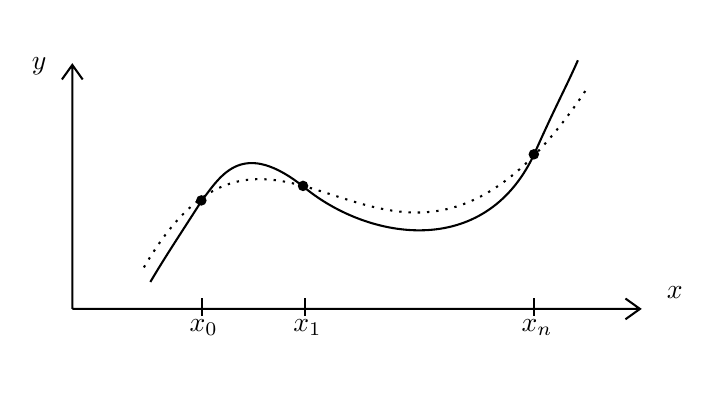
\begin{tikzpicture}[x=0.75pt,y=0.75pt,yscale=-1,xscale=1]
	%uncomment if require: \path (0,180); %set diagram left start at 0, and has height of 180

	%Shape: Axis 2D [id:dp22400730037348748]
	\draw  (168,148.78) -- (441.5,148.78)(168,31.23) -- (168,148.78) -- cycle (434.5,143.78) -- (441.5,148.78) -- (434.5,153.78) (163,38.23) -- (168,31.23) -- (173,38.23)  ;
	%Curve Lines [id:da32352899128716883]
	\draw  [dash pattern={on 0.84pt off 2.51pt}]  (202.5,128.78) .. controls (269.5,13.78) and (322.5,184.78) .. (416.5,41.78) ;
	%Straight Lines [id:da839820950039138]
	\draw    (230.33,143.67) -- (230.33,152.33) ;
	%Straight Lines [id:da7873722676835229]
	\draw    (280.33,143.67) -- (280.33,152.33) ;
	%Straight Lines [id:da8564842660802718]
	\draw    (390.33,143.67) -- (390.33,152.33) ;
	%Shape: Circle [id:dp6129946178962862]
	\draw  [fill={rgb, 255:red, 0; green, 0; blue, 0 }  ,fill opacity=1 ] (228.17,96.51) .. controls (228.17,95.4) and (229.06,94.51) .. (230.17,94.51) .. controls (231.27,94.51) and (232.17,95.4) .. (232.17,96.51) .. controls (232.17,97.61) and (231.27,98.51) .. (230.17,98.51) .. controls (229.06,98.51) and (228.17,97.61) .. (228.17,96.51) -- cycle ;
	%Shape: Circle [id:dp25002038836612006]
	\draw  [fill={rgb, 255:red, 0; green, 0; blue, 0 }  ,fill opacity=1 ] (277.17,89.51) .. controls (277.17,88.4) and (278.06,87.51) .. (279.17,87.51) .. controls (280.27,87.51) and (281.17,88.4) .. (281.17,89.51) .. controls (281.17,90.61) and (280.27,91.51) .. (279.17,91.51) .. controls (278.06,91.51) and (277.17,90.61) .. (277.17,89.51) -- cycle ;
	%Shape: Circle [id:dp7481993899672381]
	\draw  [fill={rgb, 255:red, 0; green, 0; blue, 0 }  ,fill opacity=1 ] (388.37,74.31) .. controls (388.37,73.2) and (389.26,72.31) .. (390.37,72.31) .. controls (391.47,72.31) and (392.37,73.2) .. (392.37,74.31) .. controls (392.37,75.41) and (391.47,76.31) .. (390.37,76.31) .. controls (389.26,76.31) and (388.37,75.41) .. (388.37,74.31) -- cycle ;
	%Curve Lines [id:da6764086869694204]
	\draw    (205.6,135.8) .. controls (212.4,124.2) and (220.4,112.2) .. (230.33,96.67) .. controls (239.6,84.6) and (249.87,65.94) .. (280.33,90.67) .. controls (310.8,115.4) and (366.27,125.14) .. (390.33,74.67) .. controls (401.2,50.2) and (405.6,42.6) .. (411.6,29) ;

	% Text Node
	\draw (147,26.4) node [anchor=north west][inner sep=0.75pt]    {$y$};
	% Text Node
	\draw (453,136.4) node [anchor=north west][inner sep=0.75pt]    {$x$};
	% Text Node
	\draw (223,152.4) node [anchor=north west][inner sep=0.75pt]    {$x_{0}$};
	% Text Node
	\draw (273,152.4) node [anchor=north west][inner sep=0.75pt]    {$x_{1}$};
	% Text Node
	\draw (383,152.4) node [anchor=north west][inner sep=0.75pt]    {$x_{n}$};
	\end{tikzpicture}
	\caption{Esistono diverse possibilità che rispettano le condizioni di passaggio nei nodi, è importante formalizzare delle strategie e dei criteri per determinare la migliore interpolazione.}
\end{figure}
\FloatBarrier

\begin{theorem}
Dati $n+1$ punti distinti $x_{0} ,x_{1} ,\dotsc ,x_{n}$, detti nodi di interpolazione, e $n+1$ corrispondenti valori $y_{0} ,y_{1} ,\dotsc ,y_{n}$, allora esiste un unico polinomio di interpolazione $\Pi _{n}(x)$ di grado $n$ tale che
\begin{equation}
\Pi _{n}( x_{i}) =y_{i} \quad \forall i=0,\dotsc ,n.
\label{eq:condizione-pol-interpolazione}
\end{equation}
\end{theorem}
\textbf{NB.}
Per giustificare intuitivamente il fatto che servano $n+1$ punti, ricordiamo che esiste una e una sola retta (polinomio di grado 1) passante per due punti, mentre esistono infinite parabole (polinomio di grado 2) passanti per due punti. Pertanto per fissare il nostro oggetto di grado $n$ ci servono $n+1$ punti.

\textit{Dimostrazione.} La dimostrazione è costruttiva, ovvero contiene il modo operativo per calcolare il polinomio di interpolazione. Dobbiamo mostrare che questo esista e che sia unico.

\textit{Esistenza.} Forniamo una rappresentazione esplicita del polinomio $\Pi _{n}$. Abbiamo bisogno di costruire una base per lo spazio dei polinomi di grado $n\rightarrow \mathbb{P}^{n}$ definiti su $\mathbb{R}$. Una scelta molto semplice è utilizzare la base dei monomi
\begin{equation*}
\mathbb{P}^{n} =\operatorname{span}\left\{1,x,x^{2} ,\dotsc ,x^{n}\right\} ,
\end{equation*}
cioè scrivere $\Pi _{n}(x)$ come
\begin{equation*}
\Pi _{n}(x) =a_{0} +a_{1} x+a_{2} x^{2} +\dotsc +a_{n} x^{n} ,
\end{equation*}
con $a_{0} ,a_{1} ,\dotsc ,a_{n} \in \mathbb{R}$ da determinare imponendo i vincoli di passaggio \eqref{eq:condizione-pol-interpolazione}. Costruiamo quindi una nuova base, detta \textbf{base di Lagrange}\index{base!di Lagrange}:
\begin{equation*}
\mathbb{P}^{n} =\operatorname{span}\{\mathcal{L}_{0}(x) ,\dotsc ,\mathcal{L}_{n}(x)\}
\end{equation*}
dove per ogni $i=0,\dotsc ,n$ l'$i$-esimo \textbf{polinomio di Lagrange}\index{polinomio!di Lagrange} $\mathcal{L}_{i}(x)$ è definito in modo da soddisfare le seguenti condizioni:
\begin{equation*}
\begin{array}{{>{\displaystyle}l}}
\mathcal{L}_{i}(x) \ \text{è un polinomio di grado} \ n\\
\mathcal{L}_{i}(x) =\begin{cases}
1 & \text{se} \ x=x_{i}\\
0 & \text{se} \ x=x_{j} ,\ j\neq i.
\end{cases}
\end{array}
\end{equation*}
L'espressione analitica di ogni $\mathcal{L}_{i}(x) ,i=0,\dotsc ,n$ è:
\begin{equation*}
\mathcal{L}_{i}(x) =\prod ^{n}_{j=0,j\neq i}\frac{( x-x_{j})}{( x_{i} -x_{j})} \quad i=0,\dotsc ,n,
\end{equation*}
in quanto il numeratore si annulla in ogni $x_j$ con $j\ne i$, mentre il denominatore coincide con il numeratore calcolato in $x_i$.

In figura \ref{fig-polinomi-lagrange} si può vedere un esempio di un set di polinomi di Lagrange costruiti su un specifico insieme di nodi.
\fg[Polinomi di Lagrange nei nodi $x_{i}=1,3,4,6,8$.]{0.75}{fig-polinomi-lagrange}

Si può dimostrare che questi polinomi sono indipendenti e che quindi costituiscono una base per i polinomi $\mathbb{P}^{n}$. Con questa base è immediato costruire il polinomio di interpolazione $\Pi _{n}(x)$, infatti:
\begin{equation*}
\Pi _{n}(x) =y_{0}\mathcal{L}_{0}(x) +y_{1}\mathcal{L}_{1}(x) +\dotsc +y_{n}\mathcal{L}_{n}(x).
\end{equation*}
Ovvero in forma compatta otteniamo:
\begin{equation*}
\Pi _{n}(x) =\sum ^{n}_{i=0} y_{i}\mathcal{L}_{i}(x) .
\end{equation*}
Questo ne dimostra l'esistenza.

\textit{Unicità.} Per assurdo supponiamo che esistano due polinomi di grado $n$ distinti $\Pi _{n}(x)$ e $\tilde{\Pi }_{n}(x)$ che rispettino le proprietà richieste, ovvero:
\begin{equation*}
\Pi _{n}( x_{i}) =y_{i} \quad \forall i=0,\dotsc ,n \quad \text{e} \quad \tilde{\Pi }_{n}( x_{i}) =y_{i} \quad \forall i=0,\dotsc ,n.
\end{equation*}
Definiamo ora $\mathcal{Y}_{n}(x) \coloneqq \Pi _{n}(x) -\tilde{\Pi }_{n}(x)$, che chiaramente è un polinomio di grado $n$ ed è nullo su tutti i nodi interpolazione. Abbiamo $\forall i=0,\dotsc ,n$:
$$
	\mathcal{Y}_{n}( x_{i})
	=\Pi _{n}( x_{i}) -\tilde{\Pi }_{n}( x_{i})
	=y_{i} -y_{i}
	=0.
$$
Quindi $\mathcal{Y}_{n}(x)$ è un polinomio di grado $n$ che ha $n+1$ zeri. Per il teorema fondamentale dell'algebra un polinomio di grado $n$ ha al più $n$ zeri, dunque non può che essere:
\begin{equation*}
\mathcal{Y}_{n}(x) \equiv 0\ \ \Rightarrow \ \ \Pi _{n}(x) \equiv \tilde{\Pi }_{n}(x)
\end{equation*}
ma questo è assurdo in quanto si è supposto fossero distinti, pertanto abbiamo dimostrato l'unicità. \textqed

Dal teorema abbiamo anche imparato a costruire il \textbf{polinomio di interpolazione di Lagrange}\index{polinomio!di interpolazione di Lagrange}:
\begin{equation*}
\Pi _{n}(x) =\sum ^{n}_{i=0} y_{i}\mathcal{L}_{i}(x).
\end{equation*}
Se al posto di avere le coppie di punti $\{( x_{i} ,y_{i})\}^{n}_{i=0}$ avessimo una funzione $f$ da interpolare, potremmo scrivere analogamente
\begin{equation*}
\Pi _{n} f(x) =\sum ^{n}_{i=0} f( x_{i})\mathcal{L}_{i}(x).
\end{equation*}
\textit{Osservazioni.}
\begin{itemize}
\item Le espressioni dei polinomi della base di Lagrange $\mathcal{L}_{0}(x) ,\dotsc ,\mathcal{L}_{n}(x)$ dipendono \textit{solo} dai nodi di interpolazione $x_{i} ,i=0,\dotsc ,n$.
\item Si può anche dimostrare che i polinomi di Lagrange soddisfano
\begin{equation*}
\mathcal{L}_{i}(x) =\frac{w_{n+1}(x)}{( x-x_{i}) w'_{n+1}( x_{i})} \qquad \forall i=0,\dotsc ,n
\end{equation*}
dove $w_{n+1}(x)$ è detto \textbf{polinomio nodale}\index{polinomio!nodale} ed è definito come
\begin{equation*}
w_{n+1}(x) =\prod ^{n}_{i=0}( x-x_{i}).
\end{equation*}
Ne consegue che
\begin{equation*}
\Pi _{n}(x) =\sum\limits ^{n}_{i=0} y_{i}\frac{w_{n+1}(x)}{( x-x_{i}) w'_{n+1}( x_{i})}.
\end{equation*}
\item Per trovare il polinomio di interpolazione, sarebbe anche possibile risolvere un sistema che imponga il passaggio per i punti campionati:
\begin{equation*}
    \begin{cases}
        a_0 +a_1x_0+\dots+a_nx_0^n=y_0\\
        \ \vdots \\
        a_0+a_1x_n+\dots+a_nx_n^n=y_n
    \end{cases}
    \iff
    \begin{bmatrix}
        1 & x_0 & \cdots & x_0^n\\
        \vdots&\vdots&\ddots&\vdots\\
        1 & x_n & \cdots & x_n^n
    \end{bmatrix}
    \begin{bmatrix}
        a_0\\
        \vdots\\
        a_n
    \end{bmatrix}=
    \begin{bmatrix}
        y_0\\
        \vdots\\
        y_n
    \end{bmatrix}
\end{equation*}
La matrice del sistema si chiama \textbf{matrice di Vandermonde}\index{matrice!di Vandermonde} ed è non singolare se gli $x_i$ sono distinti. Questo metodo tuttavia è difficilmente percorribile perché la matrice è mal condizionata.
\end{itemize}
\begin{theorem}
[Errore di interpolazione]
\index{errore!di interpolazione}
Siano $x_{0} ,x_{1} ,\dotsc ,x_{n}$ un set di $n+1$ punti distinti in $I\subseteq \mathbb{R}$ e sia $f\in C^{n+1}(I)$. Per ogni $x\in I$, $\exists \xi = \xi(x)\in I$ tale che l'errore $E(x) =f(x) -\Pi _{n} f(x)$ sia dato da
\begin{equation*}
E(x) =\frac{\omega _{n+1}(x)}{( n+1) !} f^{( n+1)}( \xi )
\end{equation*}
dove $\omega _{n+1}(x)$ è il polinomio nodale associato ai nodi $x_{0} ,x_{1} ,\dotsc ,x_{n}$, ossia $\omega _{n+1}(x) =\prod ^{n}_{i=0}( x-x_{i})$.
\end{theorem}

Per capire l'utilizzo del teorema, diamo la seguente definizione.
\begin{definition}
	[Norma infinito]
	\index{norma!infinito}
	Data $f$ una funzione definita su un insieme $A$, denotiamo la sua norma infinito con\footnote{La definizione esatta è in realtà più complessa, ma coinvolge concetti come misurabilità e insiemi di misura nulla, che non sono oggetto di questo libro e non necessari per la comprensione della materia.}
	\begin{equation*}
		\Vert f\Vert _{\infty} =\max_{x\in A} \left|f(x)\right|.
	\end{equation*}
\end{definition}
% (E INVECE) Abbiamo voluto dare la definizione completa, che sarà utile in vista di corsi successivi. In generale, quando diciamo `misurabile' intendiamo `misurabile secondo Lebesgue'; non è necessario approfondire per comprendere ciò che si dirà, è sufficiente dire che è una nozione più generalizzata della misurabilità secondo Riemann e che tutti le funzioni che considereremo saranno Lebesgue-misurabili. Il `q.o.' significa `quasi ovunque', ovvero a meno di insiemi di misura nulla: ciò significa che se consideriamo come funzione una parabola $f(x)=-x^2+1,\forall x\neq 0$ con $f(x)=5$ se $x=0$, anche se il suo massimo `reale' è $5$, ciò vale in un punto, che rispetto alla retta ha misura nulla. Quindi possiamo `trascurare' gli insiemi di misura nulla e dire che la sua norma infinito sull'insieme $A=\mathbb{R}$ è proprio $1$.

L'utilizzo della norma infinito è fondamentale in quanto la formula dell'errore è valida quando la funzione viene valutata in un punto $\xi$, ma questo punto non è noto, e si sa solo che esso appartiene all'intervallo $I$.
Possiamo naturalmente maggiorare il valore che la $f^{(n+1)}$ assume in $\xi$ con il massimo valore assunto nell'intervallo. Questo avviene proprio grazie alla norma infinito, che essendo un massimo su $x$ è una costante rispetto a $x$:
\begin{equation*}
| E(x)| \leqslant \frac{1}{( n+1) !} \ | \omega _{n+1}(x)| \ \underbrace{\left\Vert f^{( n+1)}(x)\right\Vert _{\infty }}_{\leqslant C} \leqslant \frac{C}{( n+1) !} \ | \omega _{n+1}(x)|\ \ \forall x\in I.
\end{equation*}

\textit{Dimostrazione.}
Fissando $x\in I$, vogliamo stimare $E(x) =f(x) -\Pi _{n} f(x)$. Abbiamo due casi:
\begin{itemize}
\item Se $x$ coincide con uno dei nodi di interpolazione, ossia $x=x_{i}$ per qualche $i$, allora il risultato è banale perché $E(x) =0$ dal momento che
\begin{equation*}
E(x) =\frac{\omega _{n+1}(x)}{( n+1) !} f^{( n+1)}( \xi ) =\frac{\prod\nolimits ^{n}_{i=0}\overbrace{( x-x_{i})}^{=0}}{( n+1) !} f^{( n+1)}( \xi ).
\end{equation*}
\item Se $x$ \textit{non} coincide con uno dei nodi di interpolazione, definiamo la seguente funzione:
\begin{equation*}
G:I\rightarrow \mathbb{R} \quad G(t) =E_{n}(t) -\omega _{n+1}(t)\frac{E_{n}(x)}{\omega _{n+1}(x)}.
\end{equation*}

Osserviamo che:
\begin{itemize}
\item $G(t) \in C^{n+1}(I)$ perché $f\in C^{n+1}(I)$ e $\omega _{n+1}(t)$ è un polinomio, quindi anch'esso è infinitamente derivabile.
\item $G(t)$ ha almeno $n+2$ zeri nell'intervallo $I$; infatti, $\forall i=0,\dotsc ,n$:
\begin{align*}
	G( x_{i}) =\underbrace{E_{n}( x_{i})}_{=0} -\underbrace{\omega _{n+1}( x_{i})}_{=0}\frac{E_{n}(x)}{\omega _{n+1}(x)} & \quad \rightarrow \quad n+1 \text{ zeri} \\
	G(x) =E_{n}(x) -\omega _{n+1}(x)\frac{E_{n}(x)}{\omega _{n+1}(x)} =0 & \quad \rightarrow \quad 1 \text{ zero.}
\end{align*}
\end{itemize}

Quindi $G(t)$ è una funzione di classe $C^{n+1}$ in $I$ con almeno $n+2$ zeri distinti. Quindi per il teorema del valor medio possiamo concludere che $G'(t)$ ha almeno $n+1$ zeri distinti e, con lo stesso ragionamento, che $G^{( n+1)}(t)$ ammette uno zero che chiamiamo $\xi =\xi (x)$, cioè $G^{( n+1)}( \xi ) =0$.

Adesso calcoliamo l'espressione di $G^{( n+1)}(t)$. Per linearità della derivata si ha:
\begin{align*}
G^{( n+1)}(t) & =E^{( n+1)}_{n}(t) -\omega ^{( n+1)}_{n+1}(t)\frac{E_{n}(x)}{\omega _{n+1}(x)}\\
 & =f^{( n+1)}(t) -\underbrace{( \Pi _{n} f)^{( n+1)}(t)}_{=0} -\underbrace{\omega ^{( n+1)}_{n+1}(t)}_{=( n+1) !}\frac{E_{n}(x)}{\omega _{n+1}(x)}\\
 & =f^{( n+1)}(t) -( n+1) !\frac{E_{n}(x)}{\omega _{n+1}(x)}.
\end{align*}

Valutiamo infine il polinomio in $\xi$:
\begin{align*}
\underbrace{G^{( n+1)}( \xi )}_{=0} & =f^{( n+1)}( \xi ) -( n+1) !\frac{E_{n}(x)}{\omega _{n+1}(x)}\\
0 & =f^{( n+1)}( \xi ) -( n+1) !\frac{E_{n}(x)}{\omega _{n+1}(x)}\\
E_{n}(x) = & \frac{\omega _{n+1}(x)}{( n+1) !} f^{( n+1)}( \xi ).
\qed
\end{align*}
\end{itemize}

\section{Utilizzo di nodi equispaziati}
\index{nodi!equispaziati}
Una proprietà desiderabile per un polinomio di interpolazione $\Pi _{n} f(x)$ è che l'errore tenda a zero se $n\rightarrow \infty $.

Ipotizziamo di approssimare la funzione nell'intervallo $I=[x_0,x_n]$ usando $n+1$ nodi equispaziati $\{x_i\}_{i=0}^n$. L'intervallo tra ciascuno dei nodi è $h=(x_n-x_0)/n$.
\begin{figure}[htpb]
	\centering
	\tikzset{every picture/.style={line width=0.75pt}} %set default line width to 0.75pt

	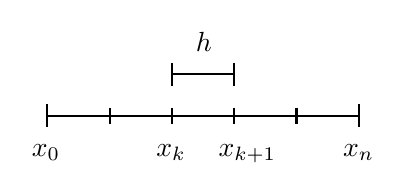
\begin{tikzpicture}[x=0.75pt,y=0.75pt,yscale=-1,xscale=1]
	%uncomment if require: \path (0,102); %set diagram left start at 0, and has height of 102

	%Straight Lines [id:da20621224248267156]
	\draw    (250,30) -- (280,30) ;
	\draw [shift={(280,30)}, rotate = 180] [color={rgb, 255:red, 0; green, 0; blue, 0 }  ][line width=0.75]    (0,5.59) -- (0,-5.59)   ;
	\draw [shift={(250,30)}, rotate = 180] [color={rgb, 255:red, 0; green, 0; blue, 0 }  ][line width=0.75]    (0,5.59) -- (0,-5.59)   ;
	%Straight Lines [id:da9554369535839922]
	\draw    (190,50) -- (340,50) (220,46) -- (220,54)(250,46) -- (250,54)(280,46) -- (280,54)(310,46) -- (310,54) ;
	\draw [shift={(340,50)}, rotate = 180] [color={rgb, 255:red, 0; green, 0; blue, 0 }  ][line width=0.75]    (0,5.59) -- (0,-5.59)   ;
	\draw [shift={(190,50)}, rotate = 180] [color={rgb, 255:red, 0; green, 0; blue, 0 }  ][line width=0.75]    (0,5.59) -- (0,-5.59)   ;

	% Text Node
	%\draw (187,22.4) node [anchor=north west][inner sep=0.75pt]    {$x_0$};
	% Text Node
	%\draw (337,22.4) node [anchor=north west][inner sep=0.75pt]    {$x_n$};
	% Text Node
	\draw (181,62.4) node [anchor=north west][inner sep=0.75pt]    {$x_0$};
	% Text Node
	\draw (241,62.4) node [anchor=north west][inner sep=0.75pt]    {$x_{k}$};
	% Text Node
	\draw (271,62.4) node [anchor=north west][inner sep=0.75pt]    {$x_{k+1}$};
	% Text Node
	\draw (260,8) node [anchor=north west][inner sep=0.75pt]    {$h$};
	% Text Node
	\draw (331,62.4) node [anchor=north west][inner sep=0.75pt]    {$x_{n}$};


	\end{tikzpicture}
\end{figure}

I nodi sono definiti da 
\begin{equation*}
    x_{i}=x_0+ih,\quad i=0,\dots,n
\end{equation*}

È possibile dimostrare che per i nodi equispaziati $|\omega_{n+1}|\le \frac{h^{n+1}} 4 n!$. Valutiamo quindi l'errore massimo nell'intervallo $I$:
\begin{multline*}
    \|E_n\|_\infty=\|f(x)-\Pi_n f(x)\|_\infty \le \frac{\|\omega_{n+1}(x)\|_\infty}{(n+1)!}\| f^{(n+1)}(x) \|_\infty\\
    \le   \frac{1}{(n+1)!} \frac{h^{n+1}}{4}\ n!\ \| \!f^{(n+1)}(x) \|_\infty
    =\underbrace{\frac{h^{n+1}}{4(n+1)}}_A \ \underbrace{\| \!f^{(n+1)}(x) \|_\infty}_B
\end{multline*}
Il termine $A$ tende a $0$ per $n\to\infty$, ma non sappiamo nulla del termine $B$: se dovesse tendere a $\infty$ più velocemente di $A$, allora l'approssimazione polinomiale diventerebbe meno accurata quando usiamo polinomi di grado superiore.

\textit{Controesempio (Fenomeno di Runge).}
Consideriamo la cosiddetta funzione di Runge, definita come:
\begin{equation*}
f:[ -5,5]\rightarrow \mathbb{R} \quad f(x) =\frac{1}{1+x^{2}}.
\end{equation*}
Se si prova a interpolare la \textbf{funzione di Runge}\index{funzione!di Runge} su un set di nodi equispaziati, per $n$ che cresce si generano delle oscillazioni via via sempre più marcate, come si vede in figura \ref{fig-runge}.

\fg[Fenomeno di Runge con polinomi interpolanti di grado $n$ crescente.]{0.6}{fig-runge}

Le oscillazioni, all'aumentare del grado, peggiorano solo \textit{in prossimità degli estremi dell'intervallo}.


 Le possibili soluzioni al fenomeno di Runge sono:
\begin{enumerate}
\item Utilizzo di \textbf{nodi non equispaziati}, concentrati agli estremi, dove ci sono oscillazioni
\item Utilizzo di \textbf{nodi equispaziati o non equispaziati} ma con metodi diversi:
\begin{enumerate}
\item \textit{Interpolazione composita}: si divide l'intervallo di approssimazione in più parti calcolando su ciascun sottointervallo un polinomio interpolante di grado $n$ non elevato $\Pi ^{n}_{h} f$.
\item \textit{Approssimazione nel senso dei minimi quadrati}, un approccio diverso dall'interpolazione vista finora.
\end{enumerate}
\end{enumerate}
\section{Utilizzo di nodi non equispaziati}
\index{nodi!non equispaziati}
\subsection{Nodi di Chebyshev-Gauss-Lobatto (CGL)}
\index{nodi!di Chebyshev-Gauss-Lobatto}
Il seguente ragionamento sarà applicato all'intervallo $I=[ -1,1]$, ma esso può essere esteso a tutto $\mathbb{R}$. Consideriamo la semicirconferenza unitaria, fissando $n$ e dividendola in $n$ spicchi di ampiezza $\frac{\pi }{n}$.
Per esempio, se $n=6$ si ha:

\begin{figure}[htpb]
	\centering
	\tikzset{every picture/.style={line width=0.75pt}} %set default line width to 0.75pt

	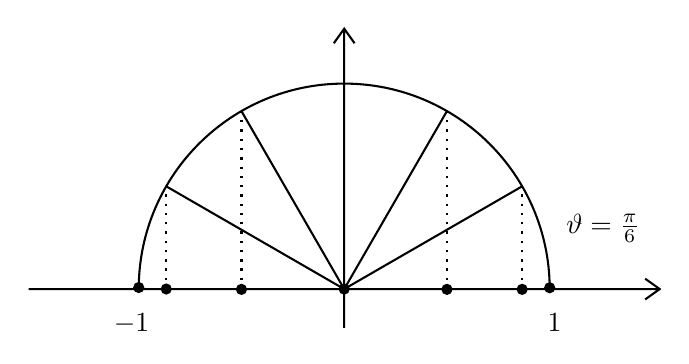
\begin{tikzpicture}[x=0.75pt,y=0.75pt,yscale=-1,xscale=1]
	%uncomment if require: \path (0,177); %set diagram left start at 0, and has height of 177

	%Shape: Axis 2D [id:dp28920976706554846]
	\draw  (147.5,134.11) -- (451.5,134.11)(299.5,8.67) -- (299.5,152.78) (444.5,129.11) -- (451.5,134.11) -- (444.5,139.11) (294.5,15.67) -- (299.5,8.67) -- (304.5,15.67)  ;
	%Shape: Circle [id:dp9498181842213234]
	\draw  [fill={rgb, 255:red, 0; green, 0; blue, 0 }  ,fill opacity=1 ] (297.33,134.11) .. controls (297.33,132.91) and (298.3,131.94) .. (299.5,131.94) .. controls (300.7,131.94) and (301.67,132.91) .. (301.67,134.11) .. controls (301.67,135.31) and (300.7,136.28) .. (299.5,136.28) .. controls (298.3,136.28) and (297.33,135.31) .. (297.33,134.11) -- cycle ;
	%Shape: Arc [id:dp9516587242954431]
	\draw  [draw opacity=0] (200.5,133.37) .. controls (200.9,79.03) and (245.07,35.11) .. (299.5,35.11) .. controls (353.96,35.11) and (398.15,79.09) .. (398.5,133.47) -- (299.5,134.11) -- cycle ; \draw   (200.5,133.37) .. controls (200.9,79.03) and (245.07,35.11) .. (299.5,35.11) .. controls (353.96,35.11) and (398.15,79.09) .. (398.5,133.47) ;
	%Shape: Boxed Line [id:dp4652733397149975]
	\draw    (299.5,134.11) -- (213.76,84.61) ;
	%Straight Lines [id:da747760306166442]
	\draw    (299.5,134.11) -- (250,48.37) ;
	%Shape: Boxed Line [id:dp3131950747001577]
	\draw    (299.5,134.11) -- (385.24,84.61) ;
	%Straight Lines [id:da26944541377482634]
	\draw    (299.5,134.11) -- (349,48.37) ;
	%Straight Lines [id:da5264596630206395]
	\draw  [dash pattern={on 0.84pt off 2.51pt}]  (349,134.25) -- (349,48.37) ;
	%Straight Lines [id:da9910633125291166]
	\draw  [dash pattern={on 0.84pt off 2.51pt}]  (385.24,134.25) -- (385.24,84.61) ;
	%Shape: Circle [id:dp28057307423967504]
	\draw  [fill={rgb, 255:red, 0; green, 0; blue, 0 }  ,fill opacity=1 ] (396.33,133.47) .. controls (396.33,132.27) and (397.3,131.3) .. (398.5,131.3) .. controls (399.69,131.3) and (400.66,132.27) .. (400.66,133.47) .. controls (400.66,134.67) and (399.69,135.64) .. (398.5,135.64) .. controls (397.3,135.64) and (396.33,134.67) .. (396.33,133.47) -- cycle ;
	%Shape: Circle [id:dp8038291186526589]
	\draw  [fill={rgb, 255:red, 0; green, 0; blue, 0 }  ,fill opacity=1 ] (198.34,133.37) .. controls (198.34,132.17) and (199.31,131.2) .. (200.5,131.2) .. controls (201.7,131.2) and (202.67,132.17) .. (202.67,133.37) .. controls (202.67,134.56) and (201.7,135.53) .. (200.5,135.53) .. controls (199.31,135.53) and (198.34,134.56) .. (198.34,133.37) -- cycle ;
	%Straight Lines [id:da9795650683884123]
	\draw  [dash pattern={on 0.84pt off 2.51pt}]  (250,134.25) -- (250,48.37) ;
	%Straight Lines [id:da5415344160854358]
	\draw  [dash pattern={on 0.84pt off 2.51pt}]  (213.76,134.25) -- (213.76,84.61) ;
	%Shape: Circle [id:dp0804362878553726]
	\draw  [fill={rgb, 255:red, 0; green, 0; blue, 0 }  ,fill opacity=1 ] (211.6,134.08) .. controls (211.6,132.89) and (212.57,131.92) .. (213.76,131.92) .. controls (214.96,131.92) and (215.93,132.89) .. (215.93,134.08) .. controls (215.93,135.28) and (214.96,136.25) .. (213.76,136.25) .. controls (212.57,136.25) and (211.6,135.28) .. (211.6,134.08) -- cycle ;
	%Shape: Circle [id:dp8087155929860674]
	\draw  [fill={rgb, 255:red, 0; green, 0; blue, 0 }  ,fill opacity=1 ] (247.83,134.25) .. controls (247.83,133.05) and (248.8,132.08) .. (250,132.08) .. controls (251.2,132.08) and (252.17,133.05) .. (252.17,134.25) .. controls (252.17,135.45) and (251.2,136.42) .. (250,136.42) .. controls (248.8,136.42) and (247.83,135.45) .. (247.83,134.25) -- cycle ;
	%Shape: Circle [id:dp21102697503346013]
	\draw  [fill={rgb, 255:red, 0; green, 0; blue, 0 }  ,fill opacity=1 ] (346.83,134.25) .. controls (346.83,133.05) and (347.8,132.08) .. (349,132.08) .. controls (350.2,132.08) and (351.17,133.05) .. (351.17,134.25) .. controls (351.17,135.45) and (350.2,136.42) .. (349,136.42) .. controls (347.8,136.42) and (346.83,135.45) .. (346.83,134.25) -- cycle ;
	%Shape: Circle [id:dp310009003820201]
	\draw  [fill={rgb, 255:red, 0; green, 0; blue, 0 }  ,fill opacity=1 ] (383.07,134.25) .. controls (383.07,133.05) and (384.04,132.08) .. (385.24,132.08) .. controls (386.43,132.08) and (387.4,133.05) .. (387.4,134.25) .. controls (387.4,135.45) and (386.43,136.42) .. (385.24,136.42) .. controls (384.04,136.42) and (383.07,135.45) .. (383.07,134.25) -- cycle ;

	% Text Node
	\draw (405,96.4) node [anchor=north west][inner sep=0.75pt]    {$\vartheta =\frac{\pi }{6}$};
	% Text Node
	\draw (187,144.4) node [anchor=north west][inner sep=0.75pt]    {$-1$};
	% Text Node
	\draw (396,144.4) node [anchor=north west][inner sep=0.75pt]    {$1$};
	\end{tikzpicture}
\end{figure}
\FloatBarrier

I nodi $x_{i}$ sono definiti come
\begin{equation}
x_{i} =-\cos\left(\frac{\pi i}{n}\right) ,\quad i=0,\dotsc ,n.
\label{eq:def-nodi-cgl}
\end{equation}
Si può dimostrare che se $f\in C^1(I)$, $\|E_{n}\|_\infty =\| \Pi _{n} f-f\|_\infty \xrightarrow{n\rightarrow \infty } 0$ con $\Pi _{n} f$ l'interpolante di Lagrange associata ai nodi di CGL.
\subsection{Nodi di Chebyshev-Gauss (CG)}
\index{nodi!di Chebyshev-Gauss}
Scegliamo solo i nodi che sono interni ad $I=[ -1,1]$, quindi tralasciando gli estremi. In questo modo:
\begin{equation}
x_{i} =-\cos\left(\frac{\pi ( 2i+1)}{2( n+1)}\right) ,\quad i=0,\dotsc ,n.
\label{eq:def-nodi-cg}
\end{equation}
Si può dimostrare che se $f$ sufficientemente regolare, $\|E_{n}\|_\infty =\| \Pi _{n} f-f\|_\infty \xrightarrow{n\rightarrow \infty } 0$ con $\Pi _{n} f$ l'interpolante di Lagrange associata ai nodi di CG.

\textbf{NB.}
Sull'intervallo generico $[ a,b]$ i nodi di CGL e CG si ottengono da \eqref{eq:def-nodi-cgl} e da \eqref{eq:def-nodi-cg} con una trasformazione lineare:
\begin{equation*}
\hat{x}_{i} =\frac{a+b}{2} +\frac{b-a}{2} x_{i}, \quad i=0,\dotsc ,n.
\end{equation*}

\section{Interpolazione composita}
\index{interpolazione!composita}
\subsection{Interpolazione composita con nodi generici}
Assegnata $f:I\rightarrow \mathbb{R}$, vogliamo approssimare $f$ usando nodi qualunque, dividendo $[ a,b]$ in sottointervalli.
\begin{enumerate}
    \item Scegliamo i nodi di interpolazione $x_0,\dots,x_M$, dividendo quindi $I$ in $M$ sottointervalli di ampiezza $h_i$
    $$I_{i} =[ x_{i} ,x_{i+1}] \quad i=0,\dotsc ,M-1, \quad h_{i} =x_{i+1}-x_i,\quad H=\max_{i}h_i.$$
    \item Su ciascun sottointervallo $I_{i}$ approssimiamo la funzione con un polinomio $\Pi ^{H}_{k} f(x)$ di interpolazione di Lagrange di grado $k\geqslant 1$, con $k$ \textit{non troppo grande} in modo da ovviare ai problemi di oscillazione.
\end{enumerate}
Quindi il polinomio di interpolazione composita $\Pi ^{H}_{k} f(x)$ soddisfa le seguenti proprietà:
\begin{itemize}
    \item $\Pi ^{H}_{k} f\in C^0([a,b])$
    \item $\Pi ^{H}_{k} f|_{I_i}\in \mathbb P^k(I_i)\quad \forall i=0,\dots ,M-1$
    \item $\Pi ^{H}_{k} f(x_i)=y_i\quad \forall i=0,\dots ,M$
\end{itemize}

\subsection{Interpolazione composita lineare}
Per $k=1$, in ogni intervallo possiamo scrivere il polinomio di interpolazione di Lagrange come
\begin{equation*}
    \Pi ^{H}_{k} f|_{I_i}(x)=f(x_i)+\frac{f(x_{i+1})-f(x_i)}{x_{i+1}-x_i}(x-x_i)
\end{equation*}
Poiché questa è un'interpolazione lineare effettuata su $2$ nodi (che essendo solo $2$ sono "equispaziati"), supponendo $f\in C^2$ possiamo usare la disuguaglianza dell'errore presentata precedentemente:
\begin{equation*}
    \|E_n\|_{\infty,I_i}=\|f(x)- \Pi ^{H}_{k} f|_{I_i}(x)\|_\infty \le \frac{h^{k+1}}{4(k+1)}\| \!f^{(k+1)}(x) \|_{\infty,I_i} = \frac{h_i^2}{8}\ \|f''(x)\|_{\infty,I_i}
\end{equation*}
Ora valutiamo l'errore nell'intero intervallo $I$, considerando il massimo che l'errore assume tra tutti gli $I_i$:
\begin{equation*}
    \|E_n\|_{\infty,I}\le \underbrace{\frac{H^2}8}_A \underbrace{\|f''(x)\|_{\infty,I}}_B
\end{equation*}
Come nel caso trattato precedentemente, il termine $A$ tende a $0$ per $M\to\infty$, ma adesso $B$ è una costante e ciò garantisce che $\|E_M\|_\infty \xrightarrow{M\to \infty}0$.
\begin{figure}[htpb]
	\centering
    \tikzset{every picture/.style={line width=0.75pt}} %set default line width to 0.75pt        
    
    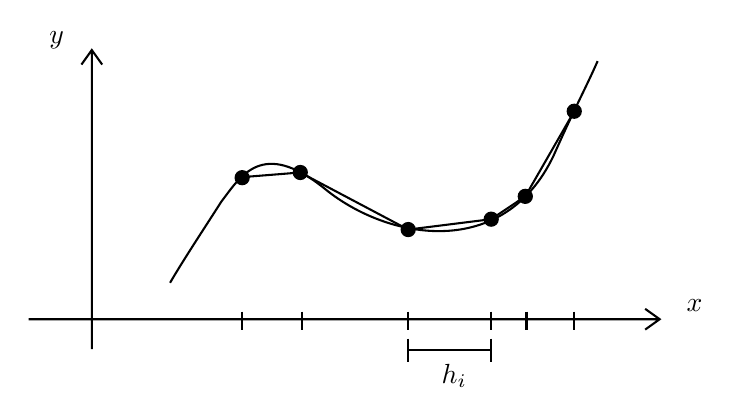
\begin{tikzpicture}[x=0.75pt,y=0.75pt,yscale=-1,xscale=1]
    %uncomment if require: \path (0,235); %set diagram left start at 0, and has height of 235
    
    %Shape: Axis 2D [id:dp18444718817100658] 
    \draw  (161.5,168.37) -- (465.5,168.37)(191.9,38.67) -- (191.9,182.78) (458.5,163.37) -- (465.5,168.37) -- (458.5,173.37) (186.9,45.67) -- (191.9,38.67) -- (196.9,45.67)  ;
    %Straight Lines [id:da062172154656692125] 
    \draw    (293.33,164.67) -- (293.33,173.33) ;
    %Shape: Circle [id:dp7214422439638635] 
    \draw  [fill={rgb, 255:red, 0; green, 0; blue, 0 }  ,fill opacity=1 ] (261.17,100.17) .. controls (261.17,98.42) and (262.58,97) .. (264.33,97) .. controls (266.08,97) and (267.5,98.42) .. (267.5,100.17) .. controls (267.5,101.92) and (266.08,103.33) .. (264.33,103.33) .. controls (262.58,103.33) and (261.17,101.92) .. (261.17,100.17) -- cycle ;
    %Shape: Circle [id:dp3795620538286856] 
    \draw  [fill={rgb, 255:red, 0; green, 0; blue, 0 }  ,fill opacity=1 ] (289.17,97.67) .. controls (289.17,95.92) and (290.58,94.51) .. (292.33,94.51) .. controls (294.08,94.51) and (295.5,95.92) .. (295.5,97.67) .. controls (295.5,99.42) and (294.08,100.84) .. (292.33,100.84) .. controls (290.58,100.84) and (289.17,99.42) .. (289.17,97.67) -- cycle ;
    %Curve Lines [id:da4712863514460399] 
    \draw    (229.6,150.8) .. controls (236.4,139.2) and (244.4,127.2) .. (254.33,111.67) .. controls (263.6,99.6) and (273.87,80.94) .. (304.33,105.67) .. controls (334.8,130.4) and (390.27,140.14) .. (414.33,89.67) .. controls (425.2,65.2) and (429.6,57.6) .. (435.6,44) ;
    %Straight Lines [id:da3752186519870171] 
    \draw    (344.33,164.67) -- (344.33,173.33) ;
    %Straight Lines [id:da4559519736586207] 
    \draw    (384.33,164.67) -- (384.33,173.33) ;
    %Straight Lines [id:da8960631674092833] 
    \draw    (264.33,164.67) -- (264.33,173.33) ;
    %Straight Lines [id:da8212422896339734] 
    \draw    (424.33,164.67) -- (424.33,173.33) ;
    %Shape: Circle [id:dp7699308608601513] 
    \draw  [fill={rgb, 255:red, 0; green, 0; blue, 0 }  ,fill opacity=1 ] (341.17,125.17) .. controls (341.17,123.42) and (342.58,122) .. (344.33,122) .. controls (346.08,122) and (347.5,123.42) .. (347.5,125.17) .. controls (347.5,126.92) and (346.08,128.33) .. (344.33,128.33) .. controls (342.58,128.33) and (341.17,126.92) .. (341.17,125.17) -- cycle ;
    %Shape: Circle [id:dp7749796192574097] 
    \draw  [fill={rgb, 255:red, 0; green, 0; blue, 0 }  ,fill opacity=1 ] (381.17,120.17) .. controls (381.17,118.42) and (382.58,117) .. (384.33,117) .. controls (386.08,117) and (387.5,118.42) .. (387.5,120.17) .. controls (387.5,121.92) and (386.08,123.33) .. (384.33,123.33) .. controls (382.58,123.33) and (381.17,121.92) .. (381.17,120.17) -- cycle ;
    %Shape: Circle [id:dp21920595374543028] 
    \draw  [fill={rgb, 255:red, 0; green, 0; blue, 0 }  ,fill opacity=1 ] (421.17,68.17) .. controls (421.17,66.42) and (422.58,65) .. (424.33,65) .. controls (426.08,65) and (427.5,66.42) .. (427.5,68.17) .. controls (427.5,69.92) and (426.08,71.33) .. (424.33,71.33) .. controls (422.58,71.33) and (421.17,69.92) .. (421.17,68.17) -- cycle ;
    %Straight Lines [id:da711773099353101] 
    \draw    (344.33,183.33) -- (384.33,183.33) ;
    \draw [shift={(384.33,183.33)}, rotate = 180] [color={rgb, 255:red, 0; green, 0; blue, 0 }  ][line width=0.75]    (0,5.59) -- (0,-5.59)   ;
    \draw [shift={(344.33,183.33)}, rotate = 180] [color={rgb, 255:red, 0; green, 0; blue, 0 }  ][line width=0.75]    (0,5.59) -- (0,-5.59)   ;
    %Straight Lines [id:da2561639103232428] 
    \draw    (384.33,120.17) -- (400.75,109.17) ;
    %Straight Lines [id:da030147884442299544] 
    \draw    (384.33,120.17) -- (344.33,125.17) ;
    %Straight Lines [id:da9060532424330414] 
    \draw    (292.33,97.67) -- (344.33,125.17) ;
    %Straight Lines [id:da9160326772746151] 
    \draw    (292.33,97.67) -- (261.17,100.17) ;
    %Straight Lines [id:da7721416652906353] 
    \draw    (401.33,164.67) -- (401.33,173.33) ;
    %Shape: Circle [id:dp5685147729949077] 
    \draw  [fill={rgb, 255:red, 0; green, 0; blue, 0 }  ,fill opacity=1 ] (397.58,109.17) .. controls (397.58,107.42) and (399,106) .. (400.75,106) .. controls (402.5,106) and (403.92,107.42) .. (403.92,109.17) .. controls (403.92,110.92) and (402.5,112.33) .. (400.75,112.33) .. controls (399,112.33) and (397.58,110.92) .. (397.58,109.17) -- cycle ;
    %Straight Lines [id:da854138099346445] 
    \draw    (400.75,109.17) -- (424.33,68.17) ;
    
    % Text Node
    \draw (170,28.4) node [anchor=north west][inner sep=0.75pt]    {$y$};
    % Text Node
    \draw (477,157.4) node [anchor=north west][inner sep=0.75pt]    {$x$};
    % Text Node
    \draw (359,188.4) node [anchor=north west][inner sep=0.75pt]    {$h_{i}$};
    
    
    \end{tikzpicture}
    
	\caption{Già nel caso di interpolazione composita con $k=1$ si può notare visivamente una maggiore \textit{precisione} nell'interpolazione, data dal fatto che stiamo lavorando su tanti intervalli di ampiezza $h_i$, pur usando un banale polinomio lineare.}
\end{figure}

\subsection{Interpolazione composita di gradi superiori al primo}
Vogliamo ora generalizzare il risultato ottenuto per l'interpolazione lineare a tratti.
Poiché un polinomio di grado superiore al primo richiede più di due nodi, all'interno di ciascun sottointervallo andiamo a scegliere ulteriori nodi, che ipotizziamo equispaziati.

In maniera analoga al caso lineare possiamo applicare in ciascun sottointervallo la stima dell'errore per nodi equispaziati, ottenendo il seguente teorema.

\begin{theorem}
Sia $f\in C^{k+1}(I)$ e sia $\Pi ^{H}_{k} f(x)$ il suo polinomio di interpolazione composita. Allora:
\begin{equation*}
\left\Vert f(x) -\Pi ^{H}_{k} f(x)\right\Vert _{\infty } \leqslant \frac{H^{k+1}}{4(k+1)} \ \left\Vert f^{( k+1)}\right\Vert _{\infty }.
\end{equation*}
\end{theorem}
\textit{Osservazione.}
Nonostante l'errore tenda a $0$ più velocemente all'aumentare di $M$, le richieste di regolarità sulla funzione sono sempre più gravose. Oltretutto la regolarità di $f$ non viene rispecchiata dal polinomio di interpolazione composita, che continua ad essere solo $C^0$. Per garantire una maggiore regolarità dell'interpolante, bisogna ricorrere a oggetti più sofisticati, come le splines.

\subsection{Splines cubiche interpolatorie}
Queste funzioni soddisfano le seguenti proprietà\footnote{
Le proprietà presentate in realtà danno origine a $4M-2$ equazioni, ma bisogna dare l'identità a $4 M$ coefficienti in quanto vanno definiti $M$ polinomi di grado $3$. Per garantire l'unicità dell'approssimazione bisognerebbe dunque aggiungere 2 condizioni.}:
\begin{itemize}
    \item $S_3(x_i)=f(x_i)\quad \forall x_i$
    \item $S_3|_{I_i}\in \mathbb P^3(I_i)\quad \forall I_ i$
    \item $S_3\in C^2(I)$
\end{itemize}

Le splines cubiche sono talmente accurate che si possono usare anche per approssimare $f'$ e $f''$.
\begin{theorem}
Sia $f$ sufficientemente regolare e sia $S_3(x)$ la sua spline cubica interpolatoria. Allora per $q=0,1,2$:
\begin{equation*}
\left\Vert f^{(q)}(x) -S_3^{(q)}(x)\right\Vert _{\infty } \leqslant C_q H^{4-q} \ \left\Vert f^{(4)}(x)\right\Vert _{\infty }
\end{equation*}
\end{theorem}


% \textit{[Lezione 11 (06-04-2020)]}
\section{Stabilità del polinomio di interpolazione}
\label{sec:stabilita-pol-interpolazione}

Sia $x_{0} ,x_{1} ,\dotsc ,x_{n}$ un insieme di $n+1$ punti distinti:

\begin{figure}[htpb]
	\centering
	\tikzset{every picture/.style={line width=0.75pt}} %set default line width to 0.75pt

	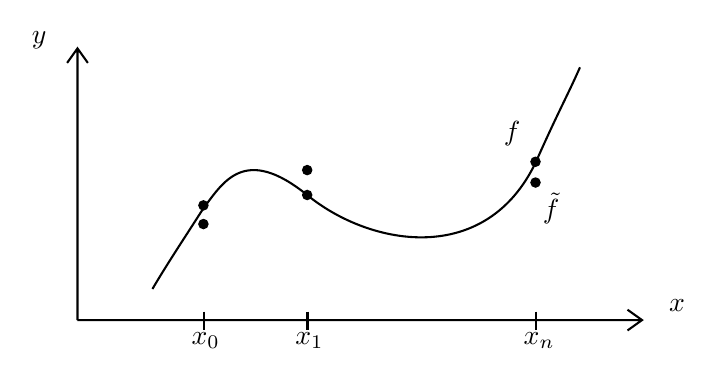
\begin{tikzpicture}[x=0.75pt,y=0.75pt,yscale=-1,xscale=1]
	%uncomment if require: \path (0,206); %set diagram left start at 0, and has height of 206

	%Shape: Axis 2D [id:dp038954507211826694]
	\draw  (169.5,167.78) -- (441.5,167.78)(169.5,36.88) -- (169.5,167.78) -- cycle (434.5,162.78) -- (441.5,167.78) -- (434.5,172.78) (164.5,43.88) -- (169.5,36.88) -- (174.5,43.88)  ;
	%Straight Lines [id:da22495486660852104]
	\draw    (230.33,163.67) -- (230.33,172.33) ;
	%Straight Lines [id:da3716248754905518]
	\draw    (280.33,163.67) -- (280.33,172.33) ;
	%Straight Lines [id:da11285799476919367]
	\draw    (390.33,163.67) -- (390.33,172.33) ;
	%Shape: Circle [id:dp13795261112398616]
	\draw  [fill={rgb, 255:red, 0; green, 0; blue, 0 }  ,fill opacity=1 ] (228.17,112.51) .. controls (228.17,111.4) and (229.06,110.51) .. (230.17,110.51) .. controls (231.27,110.51) and (232.17,111.4) .. (232.17,112.51) .. controls (232.17,113.61) and (231.27,114.51) .. (230.17,114.51) .. controls (229.06,114.51) and (228.17,113.61) .. (228.17,112.51) -- cycle ;
	%Shape: Circle [id:dp9020925580317134]
	\draw  [fill={rgb, 255:red, 0; green, 0; blue, 0 }  ,fill opacity=1 ] (278.17,107.51) .. controls (278.17,106.4) and (279.06,105.51) .. (280.17,105.51) .. controls (281.27,105.51) and (282.17,106.4) .. (282.17,107.51) .. controls (282.17,108.61) and (281.27,109.51) .. (280.17,109.51) .. controls (279.06,109.51) and (278.17,108.61) .. (278.17,107.51) -- cycle ;
	%Shape: Circle [id:dp5253082829397973]
	\draw  [fill={rgb, 255:red, 0; green, 0; blue, 0 }  ,fill opacity=1 ] (388.17,91.51) .. controls (388.17,90.4) and (389.06,89.51) .. (390.17,89.51) .. controls (391.27,89.51) and (392.17,90.4) .. (392.17,91.51) .. controls (392.17,92.61) and (391.27,93.51) .. (390.17,93.51) .. controls (389.06,93.51) and (388.17,92.61) .. (388.17,91.51) -- cycle ;
	%Curve Lines [id:da009567426004889468]
	\draw    (205.6,152.8) .. controls (212.4,141.2) and (220.4,129.2) .. (230.33,113.67) .. controls (239.6,101.6) and (249.87,82.94) .. (280.33,107.67) .. controls (310.8,132.4) and (366.27,142.14) .. (390.33,91.67) .. controls (401.2,67.2) and (405.6,59.6) .. (411.6,46) ;
	%Shape: Circle [id:dp5136163342396867]
	\draw  [fill={rgb, 255:red, 0; green, 0; blue, 0 }  ,fill opacity=1 ] (228.17,121.51) .. controls (228.17,120.4) and (229.06,119.51) .. (230.17,119.51) .. controls (231.27,119.51) and (232.17,120.4) .. (232.17,121.51) .. controls (232.17,122.61) and (231.27,123.51) .. (230.17,123.51) .. controls (229.06,123.51) and (228.17,122.61) .. (228.17,121.51) -- cycle ;
	%Shape: Circle [id:dp5738347562536119]
	\draw  [fill={rgb, 255:red, 0; green, 0; blue, 0 }  ,fill opacity=1 ] (278.17,95.51) .. controls (278.17,94.4) and (279.06,93.51) .. (280.17,93.51) .. controls (281.27,93.51) and (282.17,94.4) .. (282.17,95.51) .. controls (282.17,96.61) and (281.27,97.51) .. (280.17,97.51) .. controls (279.06,97.51) and (278.17,96.61) .. (278.17,95.51) -- cycle ;
	%Shape: Circle [id:dp3104281695353788]
	\draw  [fill={rgb, 255:red, 0; green, 0; blue, 0 }  ,fill opacity=1 ] (388.17,101.51) .. controls (388.17,100.4) and (389.06,99.51) .. (390.17,99.51) .. controls (391.27,99.51) and (392.17,100.4) .. (392.17,101.51) .. controls (392.17,102.61) and (391.27,103.51) .. (390.17,103.51) .. controls (389.06,103.51) and (388.17,102.61) .. (388.17,101.51) -- cycle ;

	% Text Node
	\draw (146,27.4) node [anchor=north west][inner sep=0.75pt]    {$y$};
	% Text Node
	\draw (453,156.4) node [anchor=north west][inner sep=0.75pt]    {$x$};
	% Text Node
	\draw (223,172.4) node [anchor=north west][inner sep=0.75pt]    {$x_{0}$};
	% Text Node
	\draw (273,172.4) node [anchor=north west][inner sep=0.75pt]    {$x_{1}$};
	% Text Node
	\draw (383,172.4) node [anchor=north west][inner sep=0.75pt]    {$x_{n}$};
	% Text Node
	\draw (373.4,70.4) node [anchor=north west][inner sep=0.75pt]    {$f$};
	% Text Node
	\draw (392.17,104.91) node [anchor=north west][inner sep=0.75pt]    {$\tilde{f}$};
	% Text Node
	\draw (323,172.4) node [anchor=north west][inner sep=0.75pt]    {$\dotsc $};
	\end{tikzpicture}
\end{figure}
\FloatBarrier

Costruiamo il polinomio di interpolazione di Lagrange di $f(x)$ dato da:
\begin{equation*}
\Pi _{n} f(x) =\sum ^{n}_{i=0} f( x_{i})\mathcal{L}_{i}(x)
\end{equation*}
dove
\begin{equation*}
\mathcal{L}_{i}(x) =\prod ^{n}_{j=0,j\neq i}\frac{( x-x_{j})}{( x_{i} -x_{j})} \quad\forall i=0,\dotsc ,n.
\end{equation*}
I valori $f( x_{i})$ possono essere affetti da errori di rappresentazione al calcolatore. Consideriamo quindi il polinomio di interpolazione ottenuto perturbando le valutazioni di $f( \cdot )$ nei nodi $x_{i}$:
\begin{equation*}
\tilde{\Pi }_{n} f(x) =\sum ^{n}_{i=0}\tilde{f}( x_{i})\mathcal{L}_{i}(x).
\end{equation*}
Come si comporta l'errore di perturbazione $\Pi _{n} f(x) -\tilde{\Pi }_{n} f(x)$ per $n\rightarrow \infty $?
\begin{align*}
\Pi _{n} f(x) -\tilde{\Pi }_{n} f(x) & =\sum ^{n}_{i=0} f( x_{i})\mathcal{L}_{i}(x) -\sum ^{n}_{i=0}\tilde{f}( x_{i})\mathcal{L}_{i}(x)\\
 & =\sum ^{n}_{i=0}\mathcal{L}_{i}(x)\underbrace{\left[ f( x_{i}) -\tilde{f}( x_{i})\right].}_{\text{errore di perturbazione}}
\end{align*}
Passando ora alla norma infinito:
\begin{align*}
\left\Vert \Pi _{n} f(x) -\tilde{\Pi }_{n} f(x)\right\Vert _{\infty } & \leqslant \underbrace{\left\Vert \sum ^{n}_{i=0}\mathcal{L}_{i}(x)\right\Vert _{\infty }}_{\Lambda _{n}(x)} \cdot \underbrace{\max_{i=1,\dotsc ,n}\left| f( x_{i}) -\tilde{f}( x_{i})\right| }_{\text{dipende solo dalla perturbazione}}\\
\left\Vert \Pi _{n} f(x) -\tilde{\Pi }_{n} f(x)\right\Vert _{\infty } & \leqslant \Lambda _{n}(x) \cdot \max_{i=1,\dotsc ,n}\left| f( x_{i}) -\tilde{f}( x_{i})\right| .
\end{align*}
Notiamo che $\Lambda_{n}(x)$ dipende solo dalla distribuzione dei nodi di approssimazione.
Essa prende il nome di \textbf{costante di Lebesgue} in quanto valore noto se i nodi sono fissati, e indipendente dalla funzione approssimata. In un certo senso è il \textit{condizionamento} del problema.

Concludiamo che l'errore di perturbazione è piccolo solo se $\Lambda_{n}(x)$ è piccola. In generale, non possiamo garantirlo, in quanto cresce per $n\rightarrow +\infty $. Si può dimostrare che
\begin{itemize}
    \item prendendo i nodi di interpolazione \textit{equispaziati}:
        \begin{equation*}
            \Lambda _{n}(x) =\left\Vert \sum ^{n}_{i=0}\mathcal{L}_{i}(x)\right\Vert _{\infty } \approx \frac{2^{n+1}}{e\, n\, (\log n+\gamma )} ,\quad\gamma \approx \frac{1}{2} ,
        \end{equation*}
    quindi con questi nodi all'aumentare di $n$ il polinomio di interpolazione diventa rapidamente più sensibile alle perturbazioni ($\approx 2^n$).
    \item Per i nodi CGL, l'andamento è logaritmico:
    $$\Lambda _{n}(x) \leqslant \frac{2}{\pi }\left[\log n+\gamma +\log\frac{8}{\pi ^{2}}\right] +\frac{\pi }{72n^{2}}.$$
    \item Per i nodi CG, similmente, vale:
    $$\Lambda _{n}(x) \leqslant \frac{2}{\pi }\left[\log( n+1) +\gamma +\log\frac{8}{\pi }\right] +\frac{\pi }{72( n+1)^{2}}.$$
        
\end{itemize}

% \textit{[Lezione 12 (07-04-2020)]}
\section{Approssimazione nel senso dei minimi quadrati}
Se i dati di cui siamo in possesso sono molto numerosi, potrebbe non aver senso cercare un'interpolazione su di essi, sia per ragioni di complessità computazionale, sia per il rischio di \textit{overfitting}, cioè la creazione di un'approssimazione eccessivamente accurata dei dati quando probabilmente essi sono affetti da errore.
In un esempio bidimensionale, potrebbe essere sufficiente una retta che descrive il comportamento qualitativo di una ``nuvola'' di punti.

Sia $( x_{i} ,y_{i})$, $i=0,\dotsc ,n$ un insieme di $n+1$ coppie di punti.


\begin{figure}[htpb]
	\centering
	\tikzset{every picture/.style={line width=0.75pt}} %set default line width to 0.75pt

	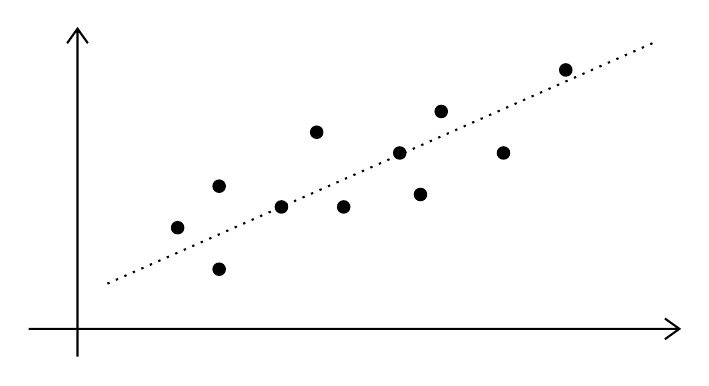
\begin{tikzpicture}[x=0.75pt,y=0.75pt,yscale=-1,xscale=1]
	%uncomment if require: \path (0,184); %set diagram left start at 0, and has height of 184

	%Shape: Axis 2D [id:dp27719212748919086]
	\draw  (146,158.49) -- (459.5,158.49)(169.5,13.88) -- (169.5,171.88) (452.5,153.49) -- (459.5,158.49) -- (452.5,163.49) (164.5,20.88) -- (169.5,13.88) -- (174.5,20.88)  ;
	%Shape: Circle [id:dp8154673289827352]
	\draw  [fill={rgb, 255:red, 0; green, 0; blue, 0 }  ,fill opacity=1 ] (215,109.75) .. controls (215,108.23) and (216.23,107) .. (217.75,107) .. controls (219.27,107) and (220.5,108.23) .. (220.5,109.75) .. controls (220.5,111.27) and (219.27,112.5) .. (217.75,112.5) .. controls (216.23,112.5) and (215,111.27) .. (215,109.75) -- cycle ;
	%Shape: Circle [id:dp2497997771583591]
	\draw  [fill={rgb, 255:red, 0; green, 0; blue, 0 }  ,fill opacity=1 ] (235,129.75) .. controls (235,128.23) and (236.23,127) .. (237.75,127) .. controls (239.27,127) and (240.5,128.23) .. (240.5,129.75) .. controls (240.5,131.27) and (239.27,132.5) .. (237.75,132.5) .. controls (236.23,132.5) and (235,131.27) .. (235,129.75) -- cycle ;
	%Shape: Circle [id:dp2629151419467781]
	\draw  [fill={rgb, 255:red, 0; green, 0; blue, 0 }  ,fill opacity=1 ] (235,89.75) .. controls (235,88.23) and (236.23,87) .. (237.75,87) .. controls (239.27,87) and (240.5,88.23) .. (240.5,89.75) .. controls (240.5,91.27) and (239.27,92.5) .. (237.75,92.5) .. controls (236.23,92.5) and (235,91.27) .. (235,89.75) -- cycle ;
	%Shape: Circle [id:dp40703778617154285]
	\draw  [fill={rgb, 255:red, 0; green, 0; blue, 0 }  ,fill opacity=1 ] (295,99.75) .. controls (295,98.23) and (296.23,97) .. (297.75,97) .. controls (299.27,97) and (300.5,98.23) .. (300.5,99.75) .. controls (300.5,101.27) and (299.27,102.5) .. (297.75,102.5) .. controls (296.23,102.5) and (295,101.27) .. (295,99.75) -- cycle ;
	%Shape: Circle [id:dp8530263048641191]
	\draw  [fill={rgb, 255:red, 0; green, 0; blue, 0 }  ,fill opacity=1 ] (265,99.75) .. controls (265,98.23) and (266.23,97) .. (267.75,97) .. controls (269.27,97) and (270.5,98.23) .. (270.5,99.75) .. controls (270.5,101.27) and (269.27,102.5) .. (267.75,102.5) .. controls (266.23,102.5) and (265,101.27) .. (265,99.75) -- cycle ;
	%Shape: Circle [id:dp3291830631551005]
	\draw  [fill={rgb, 255:red, 0; green, 0; blue, 0 }  ,fill opacity=1 ] (282,63.75) .. controls (282,62.23) and (283.23,61) .. (284.75,61) .. controls (286.27,61) and (287.5,62.23) .. (287.5,63.75) .. controls (287.5,65.27) and (286.27,66.5) .. (284.75,66.5) .. controls (283.23,66.5) and (282,65.27) .. (282,63.75) -- cycle ;
	%Shape: Circle [id:dp023574924116483986]
	\draw  [fill={rgb, 255:red, 0; green, 0; blue, 0 }  ,fill opacity=1 ] (322,73.75) .. controls (322,72.23) and (323.23,71) .. (324.75,71) .. controls (326.27,71) and (327.5,72.23) .. (327.5,73.75) .. controls (327.5,75.27) and (326.27,76.5) .. (324.75,76.5) .. controls (323.23,76.5) and (322,75.27) .. (322,73.75) -- cycle ;
	%Shape: Circle [id:dp11649449142146628]
	\draw  [fill={rgb, 255:red, 0; green, 0; blue, 0 }  ,fill opacity=1 ] (342,53.75) .. controls (342,52.23) and (343.23,51) .. (344.75,51) .. controls (346.27,51) and (347.5,52.23) .. (347.5,53.75) .. controls (347.5,55.27) and (346.27,56.5) .. (344.75,56.5) .. controls (343.23,56.5) and (342,55.27) .. (342,53.75) -- cycle ;
	%Shape: Circle [id:dp09490733528889539]
	\draw  [fill={rgb, 255:red, 0; green, 0; blue, 0 }  ,fill opacity=1 ] (332,93.75) .. controls (332,92.23) and (333.23,91) .. (334.75,91) .. controls (336.27,91) and (337.5,92.23) .. (337.5,93.75) .. controls (337.5,95.27) and (336.27,96.5) .. (334.75,96.5) .. controls (333.23,96.5) and (332,95.27) .. (332,93.75) -- cycle ;
	%Shape: Circle [id:dp2810753608488885]
	\draw  [fill={rgb, 255:red, 0; green, 0; blue, 0 }  ,fill opacity=1 ] (372,73.75) .. controls (372,72.23) and (373.23,71) .. (374.75,71) .. controls (376.27,71) and (377.5,72.23) .. (377.5,73.75) .. controls (377.5,75.27) and (376.27,76.5) .. (374.75,76.5) .. controls (373.23,76.5) and (372,75.27) .. (372,73.75) -- cycle ;
	%Shape: Circle [id:dp009238440351500232]
	\draw  [fill={rgb, 255:red, 0; green, 0; blue, 0 }  ,fill opacity=1 ] (402,33.75) .. controls (402,32.23) and (403.23,31) .. (404.75,31) .. controls (406.27,31) and (407.5,32.23) .. (407.5,33.75) .. controls (407.5,35.27) and (406.27,36.5) .. (404.75,36.5) .. controls (403.23,36.5) and (402,35.27) .. (402,33.75) -- cycle ;
	%Straight Lines [id:da3306898308124848]
	\draw  [dash pattern={on 0.84pt off 2.51pt}]  (446.5,20.88) -- (183.5,136.88) ;
	\end{tikzpicture}
\end{figure}
\FloatBarrier

Vogliamo costruire il miglior polinomio possibile $p_{m}(x)$ di grado $m< n$, che approssimi la nuvola di dati nel seguente senso:
\begin{equation}
\sum ^{n}_{i=0}( y_{i} -p_{m}( x_{i}))^{2} \leqslant \sum ^{n}_{i=0}( y_{i} -q_{m}( x_{i}))^{2} ,\quad\forall q_{m} \in \mathbb{P}^{m}.
\label{eq:condizione-min-quad}
\end{equation}
Se esiste il polinomio $p_{m}(x)$ che realizza il minimo, esso è detto polinomio di approssimazione di grado $m$ nel senso dei \textbf{minimi quadrati}.\index{minimi quadrati}

\textit{Osservazione.}
La nozione di approssimazione nel senso dei minimi quadrati è \textit{consistente} con quanto discusso fino ad ora: con $m=n$ la \eqref{eq:condizione-min-quad} diventa
\begin{equation*}
\underbrace{\sum ^{n}_{i=0}( y_{i} -\overbrace{p_{n}( x_{i})}^{\Pi _{n}( x_{i})})^{2}}_{=0} \leqslant \sum ^{n}_{i=0}( y_{i} -q_{n}( x_{i}))^{2},
\end{equation*}
ovvero otteniamo il polinomio \textit{migliore} imponendo il vincolo di passaggio su ogni singolo nodo.
Tuttavia questa scelta porta ovviamente a un polinomio di grado altissimo, e quindi fortemente instabile, come mostrato nel controesempio di Runge.
\subsection{Caso lineare}

Sia $m=1$. In tal caso si ha la \textbf{retta dei minimi quadrati}\index{retta!dei minimi quadrati} o \textbf{retta di regressione}\index{retta!di regressione}. Abbiamo $n+1$ coppie di dati $( x_{i} ,y_{i}), i=0,\dotsc ,n$. Vogliamo costruire la miglior retta possibile nell'insieme delle rette, cioè dei polinomi di primo grado. Ovvero, cerchiamo $p_{1}(x)$ tale che:
\begin{equation}
\sum ^{n}_{i=0}( y_{i} -p_{1}( x_{i}))^{2} \leqslant \sum ^{n}_{i=0}( y_{i} -q_{1}( x_{i}))^{2} ,\quad\forall q_{1} \in \mathbb{P}^{1} .
\label{eq:condizione-min-quad-1}
\end{equation}
Poiché $p_{1}(x)$ è un polinomio lineare, avrà la forma:
\begin{equation*}
p_{1}(x) =\tilde{\alpha } +\tilde{\beta } x\quad\text{con} \ \tilde{\alpha } ,\tilde{\beta } \in \mathbb{R}.
\end{equation*}
Inoltre, anche ogni altro polinomio lineare $q_{1}(x) \in \mathbb{P}^{1}$ si può scrivere come:
\begin{equation*}
q_{1}(x) =\alpha +\beta x\quad\text{con} \ \alpha ,\beta \in \mathbb{R}.
\end{equation*}
Quindi possiamo riscrivere \eqref{eq:condizione-min-quad-1}: trovare $\tilde{\alpha } ,\tilde{\beta } \in \mathbb{R}$ tali che
\begin{equation*}
\sum ^{n}_{i=0}\left( y_{i} -\left(\tilde{\alpha } +\tilde{\beta } x_{i}\right)\right)^{2} \leqslant \sum ^{n}_{i=0}( y_{i} -( \alpha +\beta x_{i}))^{2}.
\end{equation*}
Analogamente, definendo $\Phi ( \alpha ,\beta ) =\sum ^{n}_{i=0}( y_{i} -( \alpha +\beta x_{i}))^{2}$, il problema diventa trovare:
\begin{equation*}
\Phi (\tilde{\alpha } ,\tilde{\beta }) =\min_{\alpha ,\beta \in \mathbb{R}} \Phi ( \alpha ,\beta ).
\end{equation*}
Osserviamo che $\Phi ( \cdot ,\cdot )$ è un paraboloide convesso, quindi il suo unico punto di minimo si trova imponendo la condizione:
\begin{equation}
\frac{\partial \Phi ( \alpha ,\beta )}{\partial \alpha } =0 \qquad \text{e} \qquad \frac{\partial \Phi ( \alpha ,\beta )}{\partial \beta } =0.
\label{eq:condizione-min-quad-1-parab}
\end{equation}
Calcoliamo $\tilde{\alpha } ,\tilde{\beta }$ tale che \eqref{eq:condizione-min-quad-1-parab} sia soddisfatta:
\begin{equation*}
\begin{aligned}
 & \begin{cases}
\displaystyle\frac{\partial \Phi ( \alpha ,\beta )}{\partial \alpha } =\sum ^{n}_{i=0} -2( y_{i} -\alpha -\beta x_{i}) =0\\
\displaystyle\frac{\partial \Phi ( \alpha ,\beta )}{\partial \beta } =\sum ^{n}_{i=0} -2x_{i}( y_{i} -\alpha -\beta x_{i}) =0
\end{cases}\\
\Rightarrow \ \ & \begin{cases}
\displaystyle\sum ^{n}_{i=0} -2y_{i} +2\alpha +2\beta x_{i} =0\\
\displaystyle\sum ^{n}_{i=0} -2x_{i} y_{i} +2x_{i} \alpha +2\beta x^{2}_{i} =0.
\end{cases}
\end{aligned}
\end{equation*}
Abbiamo quindi ottenuto un sistema lineare di condizioni. Dividendo per $2$ e riscrivendolo in forma matriciale:
\begin{equation*}
\begin{bmatrix}
\displaystyle( n+1) & \displaystyle\sum ^{n}_{i=0} x_{i}\\
\displaystyle\sum ^{n}_{i=0} x_{i} & \displaystyle\sum ^{n}_{i=0} x^{2}_{i}
\end{bmatrix}\begin{bmatrix}
\alpha \\
\beta
\end{bmatrix} =\begin{bmatrix}
\displaystyle\sum ^{n}_{i=0} y_{i}\\
\displaystyle\sum ^{n}_{i=0} x_{i} y_{i}
\end{bmatrix}.
\end{equation*}
La soluzione $\begin{bmatrix}
\tilde{\alpha }\\
\tilde{\beta }
\end{bmatrix}$ di questo sistema lineare è il punto di minimo di $\Phi ( \alpha ,\beta )$, e fornisce quindi i coefficienti di $p_{1}(x)$. Pertanto, la retta di regressione lineare $p_{1}(x) =\tilde{\alpha } +\tilde{\beta } x$ si può calcolare attraverso la soluzione del seguente sistema lineare $( 2\times 2)$:
\begin{equation*}
\begin{bmatrix}
( n+1) & \displaystyle\sum ^{n}_{i=0} x_{i}\\
\displaystyle\sum ^{n}_{i=0} x_{i} & \displaystyle\sum ^{n}_{i=0} x^{2}_{i}
\end{bmatrix}\begin{bmatrix}
\tilde{\alpha }\\
\tilde{\beta }
\end{bmatrix} =\begin{bmatrix}
\displaystyle\sum ^{n}_{i=0} y_{i}\\
\displaystyle\sum ^{n}_{i=0} x_{i} y_{i}
\end{bmatrix}.
\end{equation*}
Osserviamo anche che la matrice è SDP, quindi il sistema ammette una e una sola soluzione come visto nei teoremi \ref{thm:esistenza-unicita-sl} e \ref{thm:A-DP-invertibile}.
\subsection{Caso generale}

Sia $m\geqslant 1$. Si può procedere come prima e riscrivere $p_{m}(x)$ come:
\begin{equation*}
p_{m}(x) =\tilde{\alpha }_{0} +\tilde{\alpha }_{1} x\ +\tilde{\alpha }_{2} x^{2} +\dotsc +\tilde{\alpha }_{m} x^{m} =\sum ^{m}_{j=0}\tilde{\alpha }_{j} x^{j} \quad \text{con} \ \tilde{\alpha }_{j} \in \mathbb{R}.
\end{equation*}
Analogamente possiamo definire un apposito funzionale e minimizzarlo:
\begin{equation*}
\min_{[ \alpha _{i} ,i=0,\dotsc ,m]} \Phi ( \alpha _{0} ,\alpha _{1} ,\dotsc ,\alpha _{m}),
\end{equation*}
ossia differenziando rispetto a tutte le variabili e ponendo le derivate uguali a zero.
Si ha il sistema di $m+1$ incognite:
\begin{equation*}
\begin{cases}
\displaystyle\frac{\partial \Phi }{\partial \alpha _{0}} =0\\
\vdots \\
\displaystyle\frac{\partial \Phi }{\partial \alpha _{m}} =0
\end{cases},
\end{equation*}
allora:
\begin{equation*}
\begin{bmatrix}
( n+1) & \sum ^{n}_{i=0} x_{i} & \dotsc  & \sum ^{n}_{i=0} x^{m}_{i}\\
\sum ^{n}_{i=0} x_{i} & \sum ^{n}_{i=0} x^{2}_{i} & \dotsc  & \sum ^{n}_{i=0} x^{m+1}_{i}\\
\vdots  & \vdots  & \ddots  & \vdots \\
\sum ^{n}_{i=0} x^{m}_{i} & \sum ^{n}_{i=0} x^{m+1}_{i} & \dotsc  & \sum ^{n}_{i=0} x^{2m}_{i}
\end{bmatrix}\begin{bmatrix}
\alpha _{0}\\
\alpha _{1}\\
\vdots \\
\alpha _{m}
\end{bmatrix} =\begin{bmatrix}
\sum ^{n}_{i=0} y_{i}\\
\sum ^{n}_{i=0} x_{i} y_{i}\\
\vdots \\
\sum ^{n}_{i=0} x^{m}_{i} y_{i}
\end{bmatrix}.
\end{equation*}
Esso è un sistema di $( m+1)$ equazioni in $( m+1)$ incognite. La matrice è SDP, quindi il sistema ammette una e una sola soluzione:
\begin{equation*}
\begin{bmatrix}
\tilde{\alpha }_{0}\\
\tilde{\alpha }_{1}\\
\vdots \\
\tilde{\alpha }_{m}
\end{bmatrix}
\end{equation*}
che è l'insieme di coefficienti che identificano il polinomio di approssimazione nel senso dei minimi quadrati.
\section{Sistemi lineari sovradeterminati}

Prendiamo un sistema lineare della forma:
\begin{equation*}
A\x =\mathbf{b}
\end{equation*}
dove $A\in \mathbb{R}^{m\times n} ,\mathbf{b} \in \mathbb{R}^{m} ,\x \in \mathbb{R}^{n}$. Il sistema si dice:
\begin{itemize}
\item \textbf{sovradeterminato}\index{sistema!sovradeterminato} se $m >n$,
\item \textbf{sottodeterminato}\index{sistema!sottodeterminato} se $m< n$.
\end{itemize}
Approfondiremo ora i sistemi sovradeterminati, caso di maggiore interesse.
Sia dunque $A\in \mathbb{R}^{m\times n} ,m\geqslant n$.
Consideriamo il sistema lineare
\begin{equation}
A\x =\mathbf{b} ,\qquad\mathbf{b} \in \mathbb{R}^{m},
\label{eq:sist-lin-sovradet}
\end{equation}
osserviamo che \eqref{eq:sist-lin-sovradet} ha soluzione nel senso classico del termine solo se il termine noto è un elemento del seguente spazio:
\begin{equation*}
\operatorname{range}(A) =\left\{\y \in \mathbb{R}^{m} \ \text{tale che} \ A\x =\y \ \text{per qualche} \ \x \in \mathbb{R}^{n}\right\}.
\end{equation*}
Dobbiamo quindi allargare il concetto di \textit{soluzione} per studiare un sistema sovradeterminato.
\begin{definition}
[Soluzione di un sistema lineare nel senso dei minimi quadrati]
\index{soluzione!ai minimi quadrati}
Dati $A\in \mathbb{R}^{m\times n}$, $m\geqslant n$, e $\mathbf{b} \in \mathbb{R}^{m}$, diciamo che $\x^{\star } \in \mathbb{R}^{n}$ è soluzione di \eqref{eq:sist-lin-sovradet} nel senso dei minimi quadrati se
\begin{equation*}
\Phi \left(\x^{\star }\right) =\min_{\x \in \mathbb{R}^{n}} \Phi (\x),
\end{equation*}
dove il funzionale da minimizzare è $\Phi (\mathbf{w}) =\Vert A\mathbf{w} -\mathbf{b}\Vert ^{2}_{2}$, il residuo nella norma euclidea.
\end{definition}
\textit{Osservazione.} Se $m=n$, la soluzione $\x^{\star }$ nel senso dei minimi quadrati coincide con la soluzione classica perché $\Phi \left(\x^{\star }\right) =0$.

Dobbiamo chiarire se la soluzione ai minimi quadrati esista e se sia unica.
\begin{lemma}
Se la soluzione $\x^{\star }$ nel senso dei minimi quadrati di un sistema lineare esiste, essa coincide con la soluzione $\x^{\star }$ nel senso classico del \textit{sistema di equazioni normali}:
\begin{equation*}
A^{T} A\x^{\star } =A^{T}\mathbf{b}.
\end{equation*}
\end{lemma}
\textit{Dimostrazione.}
Scriviamo il funzionale da minimizzare:
\begin{align*}
\Phi (\x) & =\Vert A\x -\mathbf{b}\Vert ^{2}_{2}\\
 & =( A\x -\mathbf{b})^{T}( A\x -\mathbf{b})\\
 & =\left(( A\x)^{T} -\mathbf{b}^{T}\right)( A\x -\mathbf{b})\\
 & =( A\x)^{T} A\x\underbrace{-\mathbf{b}^{T} A\x -( A\x)^{T}\mathbf{b}}_{\langle A\x ,\mathbf{b} \rangle } +\mathbf{b}^{T}\mathbf{b}\\
 & =\x^{T} A^{T} A\x -2( A\x)^{T}\mathbf{b} +\mathbf{b}^{T}\mathbf{b}\\
 & =\x^{T} A^{T} A\x -2\x^{T} A^{T}\mathbf{b} +\mathbf{b}^{T}\mathbf{b}.
\end{align*}
Calcoliamone poi il gradiente
\begin{equation*}
\nabla \Phi (\x) =2A^{T} A\x -2A^{T}\mathbf{b}
\end{equation*}
e poniamolo uguale a zero per trovare il minimo:
\begin{gather*}
\nabla \Phi \left(\x^{\star }\right) =0\\
\Updownarrow \\
A^{T} A\x^{\star } -A^{T}\mathbf{b} =0\\
\Updownarrow \\
A^{T} A\x^{\star } =A^{T}\mathbf{b}.
\end{gather*}
\begin{theorem}
Sia $A\in \mathbb{R}^{m\times n}$, $m\geqslant n$.
Se $A$ ha rango pieno, cioè $\operatorname{rank}(A) =n$, allora $A^{T} A\in \mathbb{R}^{n\times n}$ è una matrice SDP e quindi il sistema di equazioni normali
\begin{equation*}
A^{T} A\x^{\star } =A^{T}\mathbf{b}
\end{equation*}
ammette una e una sola soluzione.
\end{theorem}
\textit{Osservazione.} Se $A^{T} A\x^{\star } =A^{T}\mathbf{b}$ ammette una e una sola soluzione in senso classico, allora \eqref{eq:sist-lin-sovradet} ammette una e una sola soluzione nel senso dei minimi quadrati.

\textit{Osservazione.} In genere, la matrice $A^{T} A$ è molto mal condizionata, quindi nella pratica è spesso difficile risolvere il sistema di equazioni normali per calcolare $\x^{\star }$. Dobbiamo quindi trovare un altro modo di procedere per la risoluzione.
\subsection{Fattorizzazione QR}
Proviamo a generalizzare il concetto di fattorizzazione $LU$, visto nella sezione \ref{sec:fattorizzazione-lu} e proprio delle matrici quadrate, anche a matrici rettangolari come $A$.
\begin{definition}
[Fattorizzazione $QR$]
\index{fattorizzazione!QR}
Sia $A\in \mathbb{R}^{m\times n}$, $m\geqslant n$.
Si dice che $A$ ammette una fattorizzazione $QR$ se esistono:
\begin{itemize}
\item $Q\in \mathbb{R}^{m\times m}$ ortogonale ($Q^{-1} =Q^{T}$);
\item $R\in \mathbb{R}^{m\times n}$ trapezoidale superiore (con le righe dalla $n+1$ in poi tutte nulle) 
\end{itemize}
tali che $$A=QR$$
\end{definition}
\begin{equation*}
\underbrace{\begin{bmatrix}
\cdot  & \cdot  & \cdot \\
\cdot  & \cdot  & \cdot \\
\cdot  & \cdot  & \cdot \\
\cdot  & \cdot  & \cdot \\
\cdot  & \cdot  & \cdot
\end{bmatrix}}_{A\in \mathbb{R}^{m\times n}} =\underbrace{\begin{bmatrix}
\cdot  & \cdot  & \cdot  & \cdot  & \cdot \\
\cdot  & \cdot  & \cdot  & \cdot  & \cdot \\
\cdot  & \cdot  & \cdot  & \cdot  & \cdot \\
\cdot  & \cdot  & \cdot  & \cdot  & \cdot \\
\cdot  & \cdot  & \cdot  & \cdot  & \cdot
\end{bmatrix}}_{Q\in \mathbb{R}^{m\times m}}\underbrace{\begin{bmatrix}
\cdot  & \cdot  & \cdot \\
0 & \cdot  & \cdot \\
0 & 0 & \cdot \\
0 & 0 & 0\\
0 & 0 & 0
\end{bmatrix}}_{R\in \mathbb{R}^{m\times n}}
\end{equation*}
\textbf{Proprietà (Fattorizzazione }$QR$\textbf{ ridotta).} \index{fattorizzazione!QR!ridotta} Sia $A\in \mathbb{R}^{m\times n}$, $m\geqslant n$, di rango massimo di cui esista la fattorizzazione $QR$. Allora esiste un'unica fattorizzazione di $A$ tale che:
\begin{equation*}
A=\tilde{Q} \ \tilde{R}
\end{equation*}
dove $\tilde{Q}$ e $\tilde{R}$ sono le sottomatrici ottenute da $Q$ e $R$ nel seguente modo:
\begin{itemize}
\item $\tilde{Q} =Q( 1:m,1:n) \in \mathbb{R}^{m\times n}$;
\item $\tilde{R} =R( 1:n,1:n) \in \mathbb{R}^{n\times n}$.
\end{itemize}

Inoltre le colonne di $\tilde{Q}$ sono vettori ortonormali e $\tilde{R}$ coincide con il fattore di Cholesky della matrice $A^{T} A$, ossia $A^{T} A=\tilde{R}^{T}\tilde{R}$.
\begin{equation*}
\underbrace{\begin{bmatrix}
\cdot  & \cdot  & \cdot \\
\cdot  & \cdot  & \cdot \\
\cdot  & \cdot  & \cdot \\
\cdot  & \cdot  & \cdot \\
\cdot  & \cdot  & \cdot
\end{bmatrix}}_{A\in \mathbb{R}^{m\times n}} =\underbrace{\begin{bmatrix}
\begin{array}{|c c c|}
\hline
\cdot  & \cdot  & \cdot \\
\cdot  & \cdot  & \cdot \\
\cdot  & \tilde{Q} & \cdot \\
\cdot  & \cdot  & \cdot \\
\cdot  & \cdot  & \cdot \\
\hline
\end{array} & \begin{array}{ c }
\cdot \\
\cdot \\
\cdot \\
\cdot \\
\cdot
\end{array} & \begin{array}{ c }
\cdot \\
\cdot \\
\cdot \\
\cdot \\
\cdot
\end{array}
\end{bmatrix}}_{Q\in \mathbb{R}^{m\times m}}\underbrace{\begin{bmatrix}
\begin{array}{|c c c|}
\hline
\cdot  & \cdot  & \cdot \\
0 & \tilde{R} & \cdot \\
0 & 0 & \cdot \\
\hline
\end{array}\\
\begin{array}{ c c c }
0 & 0 & 0
\end{array}\\
\begin{array}{ c c c }
0 & 0 & 0
\end{array}
\end{bmatrix}}_{R\in \mathbb{R}^{m\times n}}
\end{equation*}
Come usiamo $A=\tilde{Q} \ \tilde{R}$ per risolvere $A\x =\mathbf{b}$?
\begin{theorem}
Sia $A\in \mathbb{R}^{m\times n}$, $m\geqslant n$, di rango massimo, e sia $\mathbf{b} \in \mathbb{R}^{m}$. Allora esiste un'unica soluzione $\x^{\star } \in \mathbb{R}^{n}$ nel senso dei minimi quadrati del sistema sovradimensionato $A\x =\mathbf{b}$ ed essa è data da:
\begin{equation*}
\x^{\star } =\tilde{R}^{-1}\tilde{Q}^{T}\mathbf{b} \qquad \text{ovvero} \qquad \tilde{R}\x^{\star } =\tilde{Q}^{T}\mathbf{b}
\end{equation*}
dove $\tilde{Q}$ ed $\tilde{R}$ sono i fattori della decomposizione ridotta di $A$.
\end{theorem}
\begin{equation*}
\underbrace{\begin{bmatrix}
\begin{array}{|c c c|}
\hline
\cdot  & \cdot  & \cdot \\
\cdot  & \cdot  & \cdot \\
\cdot  & \tilde{Q} & \cdot \\
\cdot  & \cdot  & \cdot \\
\cdot  & \cdot  & \cdot \\
\hline
\end{array} & \begin{array}{ c }
\cdot \\
\cdot \\
\cdot \\
\cdot \\
\cdot
\end{array} & \begin{array}{ c }
\cdot \\
\cdot \\
\cdot \\
\cdot \\
\cdot
\end{array}
\end{bmatrix}}_{Q\in \mathbb{R}^{m\times m}}\underbrace{\begin{bmatrix}
\begin{array}{|c c c|}
\hline
\cdot  & \cdot  & \cdot \\
0 & \tilde{R} & \cdot \\
0 & 0 & \cdot \\
\hline
\end{array}\\
\begin{array}{ c c c }
0 & 0 & 0
\end{array}\\
\begin{array}{ c c c }
0 & 0 & 0
\end{array}
\end{bmatrix}}_{R\in \mathbb{R}^{m\times n}}\underbrace{\begin{bmatrix}
\begin{array}{ c }
\cdot \\
\cdot \\
\cdot
\end{array}
\end{bmatrix}}_{\x \in \mathbb{R}^{n}} =\underbrace{\begin{bmatrix}
\begin{array}{ c }
\cdot \\
\cdot \\
\cdot \\
\cdot \\
\cdot
\end{array}
\end{bmatrix}}_{\mathbf{b} \in \mathbb{R}^{n}}
\end{equation*}
\textit{Idea di dimostrazione.} Ci concentreremo sulla dimostrazione dell'esistenza, tralasciando quella dell'unicità. Supponendo che $A$ ammetta una fattorizzazione $QR$, allora:
\begin{align*}
\Vert A\x -\mathbf{b}\Vert ^{2}_{2} & =\Vert QR\x -\mathbf{b}\Vert ^{2}_{2} & \\
 & =\left\Vert Q^{T} QR\x -Q^{T}\mathbf{b}\right\Vert ^{2}_{2} & \Vert \mathbf{z}\Vert _{2} =\left\Vert Q^{T}\mathbf{z}\right\Vert _{2} \ \forall \mathbf{z}\\
 & =\left\Vert R\x -Q^{T}\mathbf{b}\right\Vert ^{2}_{2} & \text{($Q$ è ortogonale)}\\
 & =\left\Vert \tilde{R}\x -\tilde{Q}^{T}\mathbf{b}\right\Vert ^{2}_{2} +\sum ^{m}_{i=n+1}\left[\left( Q^{T}\mathbf{b}\right)_{i}\right]^{2} & \forall \x \in \mathbb{R}^{n}.
\end{align*}
Osserviamo in particolare l'ultimo passaggio: abbiamo la norma (al quadrato, ma ciò è irrilevante) di un vettore, ovvero $R\x -Q^{T}\mathbf{b}$. Dato che la norma $2$ al quadrato è per definizione (vedi \ref{def:norma-vettore}) la somma delle componenti al quadrato, possiamo liberamente separare in due somme.
Il termine $R\x$ si separa in $\tilde{R}\x$ e una somma di zeri.
Il termine $Q^{T}\mathbf{b}$ si separa in $\tilde{Q}^{T}\mathbf{b}$ e il termine in sommatoria (si noti l'indice che va da $n+1$ a $m$).
Il minimo di $\Phi (\x)$ è raggiunto per $\x^{\star }$ che annulla tutto il termine in cui compare:
\begin{equation*}
\tilde{R}\x -\tilde{Q}^{T}\mathbf{b} =0\ \ \Rightarrow \ \ \left\Vert \tilde{R}\x -\tilde{Q}^{T}\mathbf{b}\right\Vert =0
\end{equation*}
e dunque $\x^{\star }$ soddisfa
\begin{gather*}
\tilde{R}\x^{\star } -\tilde{Q}^{T}\mathbf{b} =0\ \ \Rightarrow \ \ \x^{\star } =\tilde{R}^{-1}\tilde{Q}^{T}\mathbf{b}.
\qed
\end{gather*}
\textit{Osservazione.} Il costo di calcolare la fattorizzazione $QR$ è $\approx mn^{2}$. L'algoritmo per il calcolo di $Q$ è basato sull'algoritmo di Gram-Schmidt, la tecnica dall'algebra lineare per la costruzione di una base ortogonale.
